\documentclass{sig-alternate-05-2015}

\usepackage{amsmath}
\usepackage{color}
\usepackage{xcolor}
\usepackage{colortbl}
\usepackage{listings}
\usepackage{multirow}
\usepackage{mdframed}
\usepackage{url}
\usepackage[subsubsection]{algorithm}
\usepackage{algpseudocode}
\usepackage[numbers,sort&compress]{natbib}

\newtheorem{definition}{Definition}
\newtheorem{defn}{Definition}
\newtheorem{property}{Property}
\newtheorem{theorem}{Theorem}

\definecolor{LightCyan}{rgb}{0.88,1,1}
\definecolor{BluishGray}{RGB}{226,227,231}
\definecolor{LightGray}{gray}{0.95}
\definecolor{Gray}{gray}{0.85}
\usepackage{algpseudocode,algorithm,algorithmicx}
\usepackage{comment}
\newcommand*\DNA{\textsc{dna}}

\newcommand*\Let[2]{\State #1 $\gets$ #2}
\algrenewcommand\algorithmicrequire{\textbf{Input:}}
\algrenewcommand\algorithmicensure{\textbf{Output:}}

\usepackage{listings}



%\usepackage{enumitem}

\newcommand{\ti}{\textit}
\newcommand{\tb}{\textbf}

\lstset{
language=C++,                % choose the language of the code
basicstyle=\small,       % the size of the fonts that are used for the code
%numbers=left,                   % where to put the line-numbers
%numberstyle=\footnotesize,      % the size of the fonts that are used for the line-numbers
%stepnumber=1,                   % the step between two line-numbers. If it is 1 each line will be numbered
%numbersep=5pt,                  % how far the line-numbers are from the code
backgroundcolor=\color{white},  % choose the background color. You must add \usepackage{color}
showspaces=false,               % show spaces adding particular underscores
showstringspaces=false,         % underline spaces within strings
showtabs=false,                 % show tabs within strings adding particular underscores
%frame=single,           % adds a frame around the code
tabsize=2,          % sets default tabsize to 2 spaces
captionpos=b,           % sets the caption-position to bottom
breaklines=true,        % sets automatic line breaking
breakatwhitespace=false,    % sets if automatic breaks should only happen at whitespace
escapeinside={\%*}{*)},          % if you want to add a comment within your code
numbers=right,
numbersep=-8pt,
numberstyle=\tiny,
}

\algrenewcommand{\alglinenumber}[1]{\scriptsize#1:}

\begin{document}

% Copyright
\setcopyright{acmcopyright}
%\setcopyright{acmlicensed}
%\setcopyright{rightsretained}
%\setcopyright{usgov}
%\setcopyright{usgovmixed}
%\setcopyright{cagov}
%\setcopyright{cagovmixed}


% DOI
\doi{10.475/123_4}

% ISBN
\isbn{123-4567-24-567/08/06}

%Conference
\conferenceinfo{ASE '16}{September 3--7, 2016, Singapore}

\acmPrice{\$15.00}

%
% --- Author Metadata here ---
\conferenceinfo{ASE}{'16 Singapore}
%\CopyrightYear{2007} % Allows default copyright year (20XX) to be over-ridden - IF NEED BE.
%\crdata{0-12345-67-8/90/01}  % Allows default copyright data (0-89791-88-6/97/05) to be over-ridden - IF NEED BE.
% --- End of Author Metadata ---

\title{From UML State Machine to code and back again!}
%
% You need the command \numberofauthors to handle the 'placement
% and alignment' of the authors beneath the title.
%
% For aesthetic reasons, we recommend 'three authors at a time'
% i.e. three 'name/affiliation blocks' be placed beneath the title.
%
% NOTE: You are NOT restricted in how many 'rows' of
% "name/affiliations" may appear. We just ask that you restrict
% the number of 'columns' to three.
%
% Because of the available 'opening page real-estate'
% we ask you to refrain from putting more than six authors
% (two rows with three columns) beneath the article title.
% More than six makes the first-page appear very cluttered indeed.
%
% Use the \alignauthor commands to handle the names
% and affiliations for an 'aesthetic maximum' of six authors.
% Add names, affiliations, addresses for
% the seventh etc. author(s) as the argument for the
% \additionalauthors command.
% These 'additional authors' will be output/set for you
% without further effort on your part as the last section in
% the body of your article BEFORE References or any Appendices.

\numberofauthors{1} %  in this sample file, there are a *total*
% of EIGHT authors. SIX appear on the 'first-page' (for formatting
% reasons) and the remaining two appear in the \additionalauthors section.
%
\author{
\alignauthor
Van Cam Pham, Ansgar Radermacher, S\'ebastien G\'erard\\
       \affaddr{CEA}\\
       \affaddr{Address}\\
       \affaddr{Saclay, France}\\
       \email{first-name.last-name@cea.fr}
}
\maketitle
% TODO This needs to be updated according to the intro!!!

\begin{abstract}
Model-driven engineering (MDE) is a development methodology aiming to increase software productivity and quality by automatically generating code from higher level abstraction models. Although many tools and research prototypes can generate executable code from models such as UML, generated code could be manually modified by programmers. After code modifications, round-trip engineering (RTRIP) supported by many tools is needed to make the model and code consistent but most of the tools are only applicable to static diagrams such as classes. In this paper, we address the RTRIP of UML State Machine diagrams and code. We propose a RTRIP approach consisting of a forward process, which generates code, and a backward process, which updates the original state machine from the modified generated code. From the proposed approach, we implemented a prototype and conducted several experiments on different aspects of the round-trip engineering to verify the proposed approach.
\end{abstract}



%
% The code below should be generated by the tool at
% http://dl.acm.org/ccs.cfm
% Please copy and paste the code instead of the example below. 
%
\begin{CCSXML}
<ccs2012>
 <concept>
  <concept_id>10010520.10010553.10010562</concept_id>
  <concept_desc>Computer systems organization~Embedded systems</concept_desc>
  <concept_significance>500</concept_significance>
 </concept>
 <concept>
  <concept_id>10010520.10010575.10010755</concept_id>
  <concept_desc>Computer systems organization~Redundancy</concept_desc>
  <concept_significance>300</concept_significance>
 </concept>
 <concept>
  <concept_id>10010520.10010553.10010554</concept_id>
  <concept_desc>Computer systems organization~Robotics</concept_desc>
  <concept_significance>100</concept_significance>
 </concept>
 <concept>
  <concept_id>10003033.10003083.10003095</concept_id>
  <concept_desc>Networks~Network reliability</concept_desc>
  <concept_significance>100</concept_significance>
 </concept>
</ccs2012>  
\end{CCSXML}

\ccsdesc[500]{Computer systems organization~Embedded systems}
\ccsdesc[300]{Computer systems organization~Redundancy}
\ccsdesc{Computer systems organization~Robotics}
\ccsdesc[100]{Networks~Network reliability}
%
% End generated code
%

%
%  Use this command to print the description
%
\printccsdesc

% We no longer use \terms command
%\terms{Theory}

\keywords{Round-trip engineering, code generation, state machine, UML, C++}

%Some terms to find, define, and keep coherent:
%- Developer
%- The developer who uses models is called... (e.g. software architect modeler? doesn't mean anything)
%- The developer who uses code is called... (e.g. programmer)
%- Our method is for... called... (e.g. method for model code synchronization, method for architect/programmer collaboration, etc...)
%- Model is...
%- Code is...
%- Gap or difference ?
%- Background or practice or habits or profiles ? Maybe keep profile and choose one of the other?


\section{Introduction}
\label{sec:introduction}
Model-driven engineering (MDE) is a development methodology aiming to increase software productivity and quality by allowing different stakeholders to contribute to the system description \cite{Mussbacher2014}. MDE considers models as first-class artifacts and generates code from higher abstraction level models. Although many tools and research prototypes can generate executable code from models such as UML \cite{Specification2007}, generated code could be manually modified by programmers, e.g. skeleton code generated from UML class diagrams. Models and the generated code are therefore out of synchronization. Round-trip engineering is proposed to keep the artifacts synchronized.

Round-trip engineering \cite{Aßmann200333} (RTRIP) supports synchronizing different software artifacts, model and code in this case, and thus enabling actors (software architect and programmers) to freely move between different representations \cite{Sendall}. Tools such as for instance Enterprise Architect \cite{sparxsystems_enterprise_2014}, Visual Paradigm \cite{visual}, AndroMDA \cite{_andromda_} provide RTRIP but most of them are only applicable for system structure models such as class diagrams. The RTRIP of behavior diagrams is simply not supported by these tools since (1) RTRIP is a challenge even for structural code and there is a (2) the gap between behavior models and low level code. There are no obvious bijective mappings from behavioral models and code. Furthermore, user modifications made to the generated code are not trivial to control and reflect to the model.

This study addresses the RTRIP of UML State Machine (SM) and object-oriented programming languages such as C++ and JAVA. SM is widely used in practice for modeling the behavior of complex systems, notably reactive, real-time embedded systems. There are several approaches to generating source code from state machines or state charts such as nested switch/if statements \cite{Booch1998}, state-event-table \cite{Douglass1999, Duby2001} approach and state pattern \cite{Allegrini2002,Shalyto2006,Douglass1999}. Unfortunately, the generated code from these approaches is very difficult for programmers to maintain without an appropriate supporting tool. RTRIP is impossible in these approaches even with very small changes such as changing transition targets or actions made to code. The reason behind this impossibility is that, in mainstream programming languages such as C++, JAVA, there are not equivalents between SM and source code statements.

Synchronization of SM and code allows stakeholders to better collaborate in reactive software system development. In this paper, we propose an approach to supporting this synchronization. The approach consists of a forward and a backward process. The forward process taking as input a SM executes two transformations. The first is UML to UML by utilizing several transformation patterns such as the double-dispatch approach presented in \cite{spinke_object-oriented_2013} and the second is a generation of code from the transformed UML. During the transformations, traceability information is stored. In the backward direction, a verification is executed by code pattern detection to verify the static semantic correctness of the code before the backward process taking as input the modified generated code, the UML classes, the original SM and mapping information together merges changes from code to the SM. From the proposed approach, we implemented a prototype supporting RTRIP of SM and C++ code, and conducted several experiments on different aspects of the RTRIP to verify the proposed approach. Our implementation is the first tool supporting RTRIP of SM and code. 
%The prototype also improves the collaboration between MDE developers and traditional programmers in developing reactive complex embedded systems.

To sum up, our contribution is as followings:
\begin{itemize}
  \item An approach to round-tripping UML SMs and object-oriented code.
  \item A first tooling prototype supporting RTRIP of UML SMs and C++ code.
  \item An automatic evaluation of RTRIP correctness of the proposed approach with the prototype including 300 random generated SM models containing 80 states, more than 230 transitions, more than 250 actions and around 180 events for each.
  \item A complexity analysis of the approach and performance evaluation.
  \item A comparison and collaboration of two software development practices including working at the model level and at the code level.
  \item A lightweight evaluation of the semantic conformance of the runtime execution of generated code.
\end{itemize}

The remaining of this paper is organized as follows: Section \ref{sec:related_works} shows related work. Our proposed approach is detailed in Section \ref{sec:approach}. The implementation of the prototype is described in Section \ref{sec:implementation}. Section \ref{sec:experiments} reports our results of experimenting with the implementation and our approach. The conclusion and future work are presented in Section \ref{sec:conclusion}.


\section{Related Work}
\label{sec:related_works}
Two main topics directly related to our study are identified. One is the implementation techniques and code generation for UML SMs and the other one is RTRIP.
\subsection{Implementation and code generation for UML SMs}
Main approaches including switch/if, state table and state pattern are investigated.

Switch/if is the most intuitive technique implementing a "flat" state machine. Two types of switch/if are supported. The first one uses a scalar variable representing the current active state \cite{Booch1998}. A method for each event processes the variable as a discriminator in switch/if statement. The second one uses doubly nested switch/if and has two variables to represent the current active state and the event to be processed \cite{Douglass1999}. The latter are used as the discriminators of an outer switch statement to select between states and an inner one/if statement to decide how the event should be processed. The behavior code of the two types is put in one file or class. This practice makes code cumbersome, complex, difficult to read and less explicit when the number of states grows or the state machine is hierarchical. Furthermore, the first approach lets the code scatter in different places. Therefore, maintaining or modifying such code of complex systems is very difficult.

In \cite{Douglass1999, Duby2001} the authors also propose a double dimensional state table in which one dimension represents states and the other one all possible events. Each cell of the table is associated with a function pointer meaning that the state associated with a dimension index of the cell is triggered by the event associated with the other dimension. This technique is efficient for flat and simple state machines. As the switch/if technique, this approach gets cumbersome and non-trivial to maintain since states and events represented by indexes of the table are not explicit. Furthermore, this approach requires every transition must be triggered by at least an event. This is obviously only applied to a very small sub-set of UML state machines.  
  
State pattern \cite{Allegrini2002,Shalyto2006,Douglass1999} is an object-oriented way to implement state machines. Each state is represented as a class and each event as a method. The event processing is executed by a delegation from the state machine context class to sub-states. Separation of states in classes makes the code more readable and maintainable. Unfortunately, this technique only supports flat state machines. The authors in \cite{niaz_mapping_2004} extends this to overcome its limitations. However, the maintenance of the code generated or implemented by this approach is not trivial since it requires a lot of code to write and many small changes in different places. This is critically impractical when dealing with large state machines. Furthermore, similar to the state table, this approach also poses the requirement of having at least one event for transition.

Double-dispatch pattern is proposed in \cite{spinke_object-oriented_2013} as a new technique to implement state machines. States and events are represented as classes. Our generation approach relies on this approach. The latter provides some 1-1 mappings from state machines to object-oriented code and the implementation technique is not dependent on a specific programming language. However, the approach does not deal with triggerless transitions and different event types supported by UML such as \ti{CallEvent}, \ti{TimeEvent} and \ti{SignalEvent}. Furthermore, the proposed approach is not a code generation approach but manual implementation.

Readers of this paper are recommended referring to c\cite{Domnguez2012} for a systematic survey on different approaches generating code from state machine/state charts.

\subsection{Round-trip engineering}
RTRIP of UML models and object-oriented code are supported in many tools including research prototypes and commercial such as Enterprise Architect \cite{sparxsystems_enterprise_2014}, Visual Paradigm \cite{visual}, AndroMDA \cite{_andromda_}. Although these tools work well with UML class diagrams and code, behavioral diagrams are not well supported.  

Fujaba \cite{KNNZ99_2_ag} offers a round-trip engineering environment. An interesting part of Fujaba is that it abstracts from Java source code to UML class diagrams and a so-called story-diagrams. Java code can also be generated from these diagrams. RTRIP of these diagrams and code works but limited to the naming conventions and implementation concepts of Fujaba which are not UML-compliant. 

The authors in \cite{angyal_synchronizing_2008} propose a syntactic synchronization technique for domain-specific modeling languages (DSML) and code. The approach uses an Abstract Syntax Tree (AST) metal-model to model source. Changes in code detected by using an algorithm proposed  in \cite{Chawathe:1996:CDH:235968.233366} to compare the AST instance of the current code with the last synchronized one are merged to the instance of DSML. However, an AST is very low level and it is not clear to have mappings from DSML instances to AST instances. Furthermore, although there is an example for illustrating the technique, a systematic evaluation of the approach is not presented to show its scalability.

%Round-trip engineering of Activity diagram and code is proposed in [13]. The approach uses intermediate models to reduce the abstraction gap between diagrams and code. However, the activity diagram contains plenty of low level information such as variable declarations. Furthermore, no semantic analysis is supported.


\section{approach}
\label{sec:approach}
This section presents our RTRIP approach. At first, it sketches UML SM concepts. The outline and the detail of the approach are presented afterward.
\subsection{Background}
UML SM is widely used as a means to modeling the behavior of a component in complex, reactive systems. A SM has a number of possible states and well-defined conditional transitions between states. A state is either an atomic state, a hierarchical state that is composed of sub-states and has at most one active sub-state at a certain time, or a concurrent state which could have several active sub-states at the same time. Only one of the inner states of the SM can be active at a time. A state can have associated actions such as entry/exit/doActivity executed in the running of the SM. The active state of the machine can be changed to another state triggered by external or internal events. An action can also be activated by the trigger in transitioning from one state to another one.  

Our RTRIP approach is based on the double-dispatch pattern presented in \cite{spinke_object-oriented_2013} for mapping from UML SM to UML classes and traceability-mapping management in RTRIP. Figure \ref{fig:outline} shows the outline of our RTRIP approach consisting of a forward and a backward process. In the forward process, a SM is transformed into UML classes which contain attributes, operations and a block of text as method body associated with each implemented operation. The transformation uses several patterns which will be presented later. A tracing information table is created in the transformation to be used in the backward direction of the RTRIP. The UML classes are then used as the input of a classical code generator to create source code. This generation step also puts mapping from UML classes to object-oriented source code in a second mapping table.

In the backward (reverse) direction, when the source code is modified, a verification process checks whether the modified code conforms to the SM semantics (see Section C for the detail of the verification). The backward transformation takes as input the tracing tables, the created UML classes and the SM to update these models sequentially. While the forward process can generate code from hierarchical and concurrent SMs, the backward one only works for hierarchical machines excluding some pseudo-states which are \ti{history}, \ti{join}, \ti{fork}, \ti{choice} and \ti{junction}. These features are in future work.

\begin{figure}
\centering
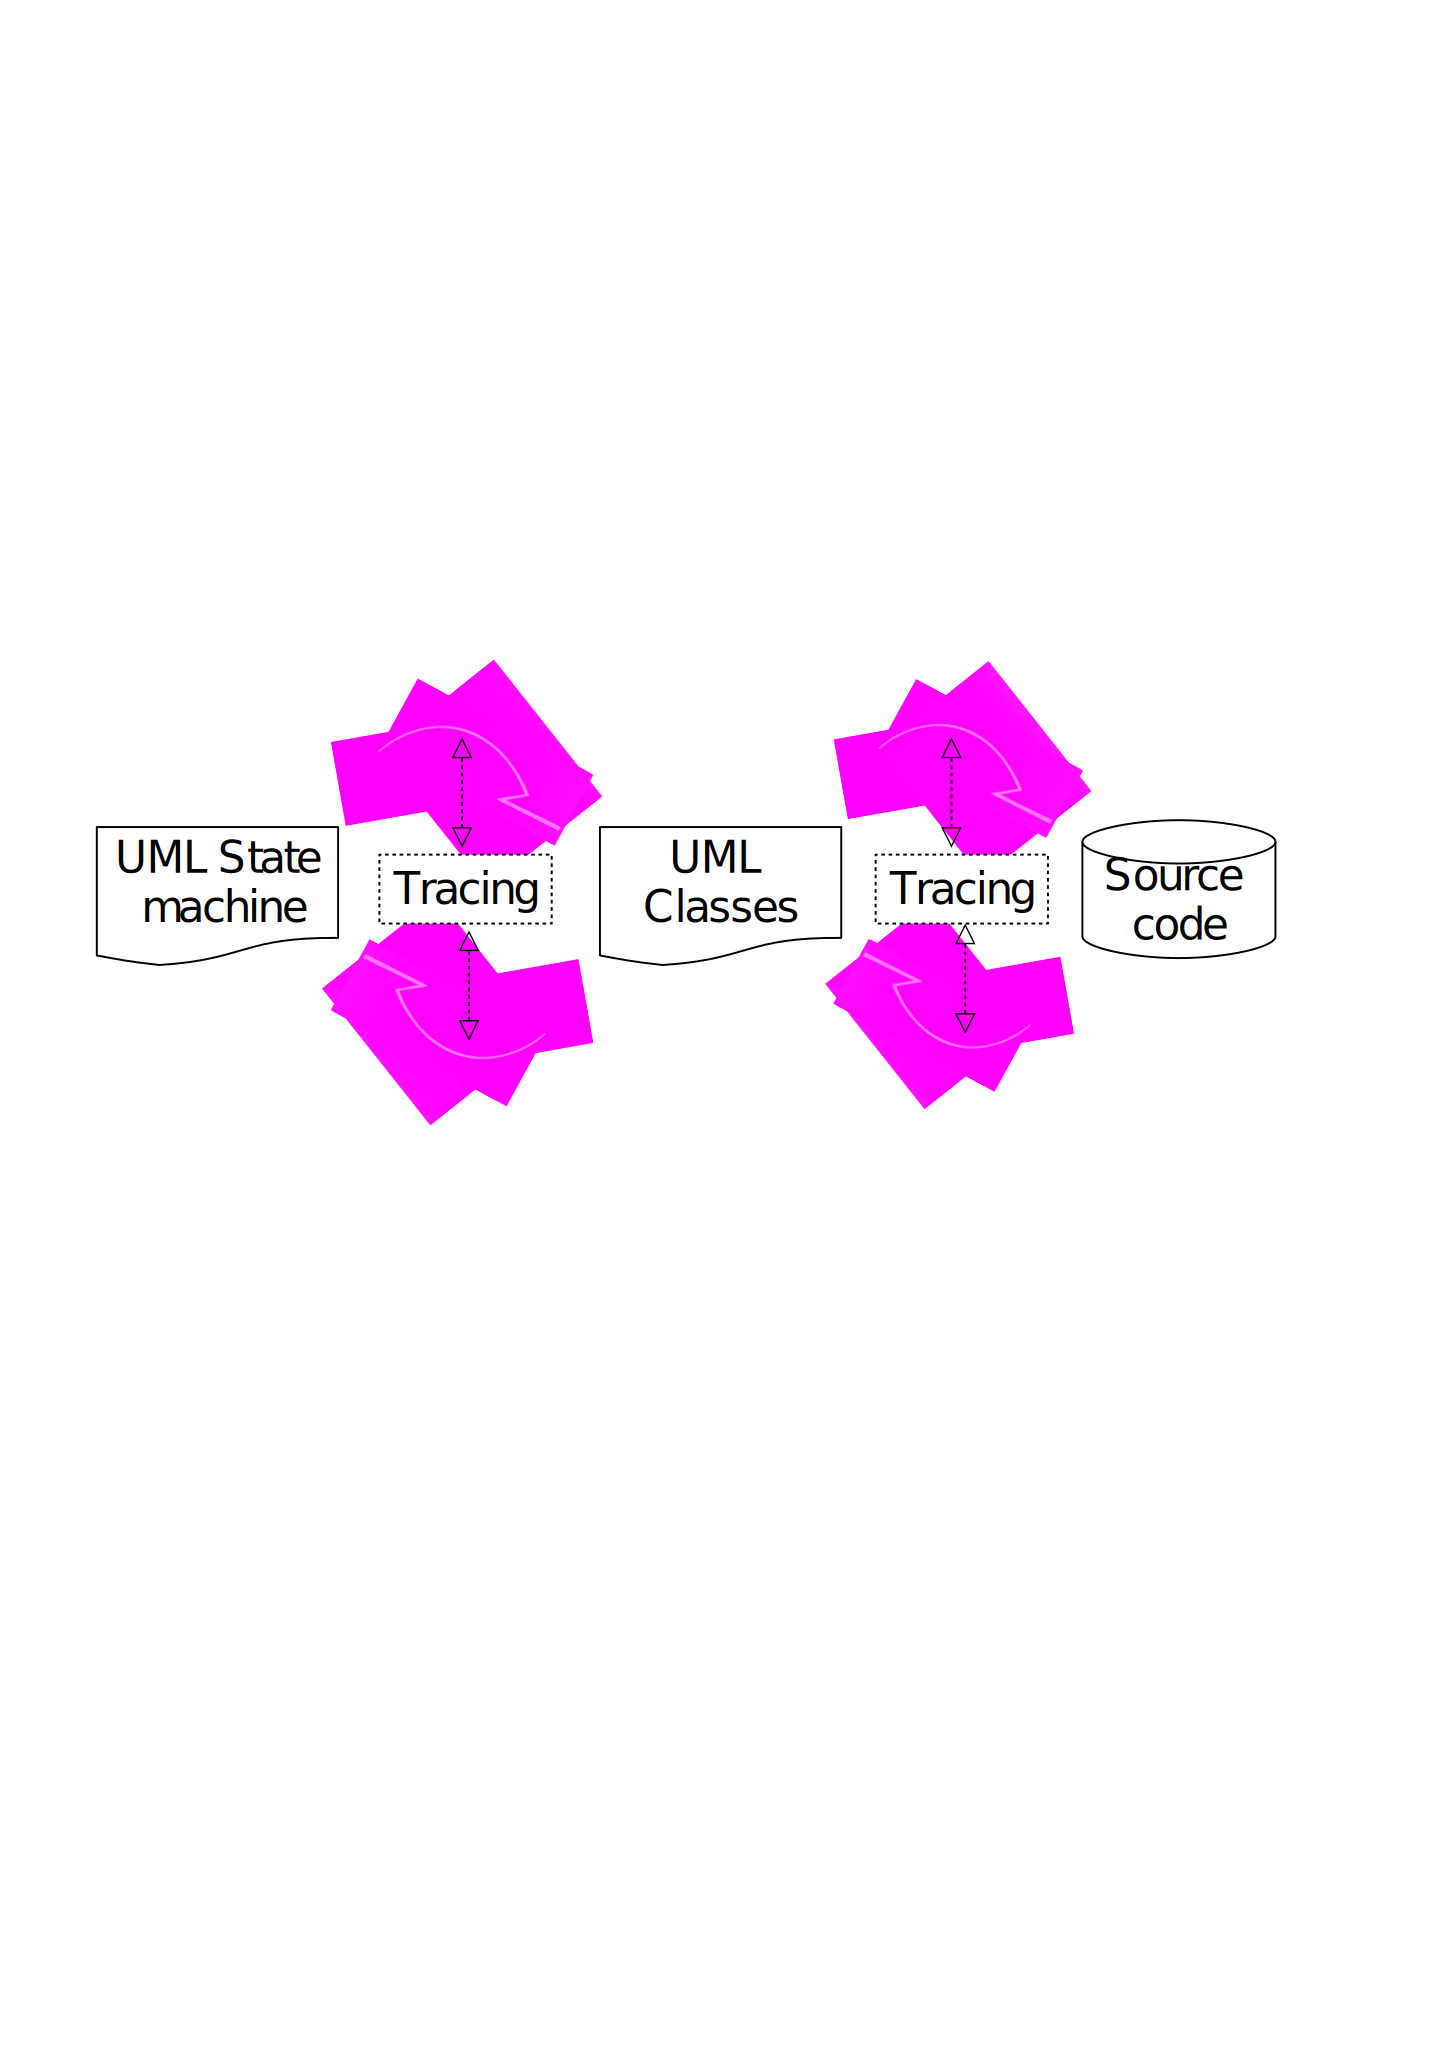
\includegraphics[clip, trim=0.5cm 10.4cm 0.5cm 7.0cm, width=0.45\textwidth]{figures/rte}
\caption{Outline of State machine and code RTE} 
\label{fig:outline}
\end{figure}

\subsection{From UML state machine to UML classes}
This section describes the forward process. The latter consists of transforming UML SM elements (see \ref{subsec:states}, \ref{subsec:events}, \ref{subsec:transitions}) into the intermediate model, storing tracing information (see \ref{subsec:trace}) and code generation (see \ref{subsec:codegen}) from the intermediate model.

\subsubsection{Transformation of states}
\label{subsec:states}
This sub-section describes the transformation of states to the intermediate model. 

This paper considers a component as a UML class called context class. Each state of the SM is transformed into a UML class in an intermediate model instead of directly generating object-oriented code as in \cite{Niaz2005}. Each UML class representing a state inherits from a base state class in the intermediate model. The base state class defines a reference to the context class, a process event operation for each event in the SM and other operations as the double-dispatch (DD) approach in \cite{spinke_object-oriented_2013}. A state class \ti{s} also has an attribute referring to the state class associated with the composite state containing \ti{s}. A composite state class has an attribute pointing to a state instance indicating the active sub-state of the composite state and a \ti{dispatchEvent} operation (see \ref{subsec:codegen}) dispatching incoming events to the appropriate active state. An example of this transformation in shown in Figure \ref{fig:hierarchical-class}. The \ti{ParentState} and \ti{SubState} are vertexes of the SM describing the \ti{Client} component, for instance. The \ti{State} and \ti{CompositeState} classes are library classes. The \ti{ParentState} inherits from the \ti{CompositeState} class since it is a hierarchical state.

\begin{figure}
\centering
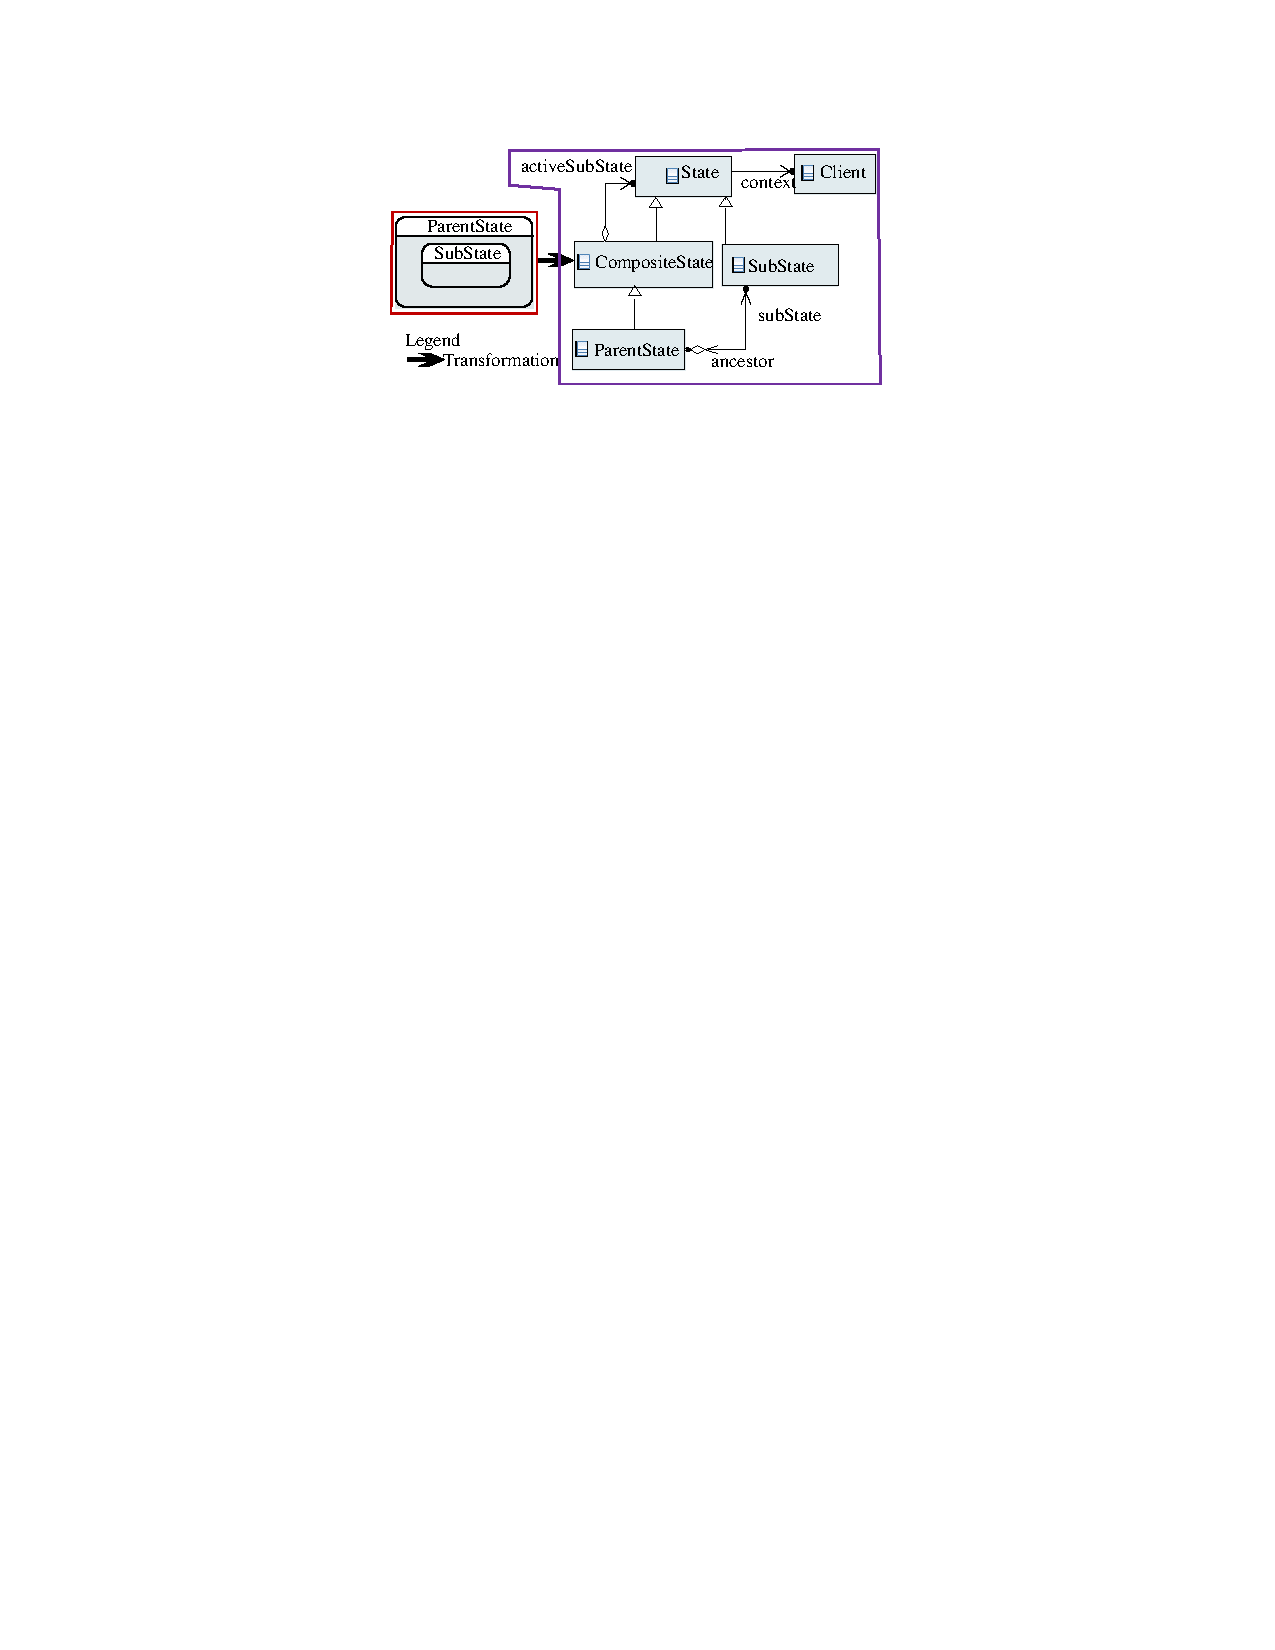
\includegraphics[clip, trim=6.5cm 21.3cm 0.5cm 2.4cm, width=0.8\textwidth]{figures/compositepattern}
\caption{Transformation from hierarchical state to class diagram} 
\label{fig:hierarchical-class}
\end{figure}

\subsubsection{Transformation of events}
\label{subsec:events}
DD has no means to convey data of events in the SM and considers every event as the same. In our approach, each event is transformed into a UML class that can contain data. Three different event class types corresponding to the UML event types \ti{CallEvent}, \ti{SignalEvent} and \ti{TimeEvent} are differentiated. An event class associated with a \ti{CallEvent} inherits from the base event class and contains the parameters in form of attributes typed by the same types as those of the operation associated with the \ti{CallEvent}. The operation must be a member of the provided interface of a port of the context class (a component as described above). For example, a call event \ti{CallEventSend} associated with an operation named Send, which has two input parameters typed by Integer, is transformed into a class \ti{CallEventSend} having two attributes typed by \ti{Integer}. When a component receives an event, the event object is stored in an event queue.

A signal event enters the component through a port typed by the signal. From the implementation view, this signal is transferred to the component by an operation provided by the component at the associated port. Therefore, the transfer of a signal event becomes similar to that of \ti{CallEvent}. For example, a signal event containing a data \ti{SignalData} arrives at a port p of a component C. The transformation derives an interface \ti{SignalDataInterface} existing as the provided interface of p. \ti{SignalDataInterface} has only one operation \ti{pushSignalData} whose body will be generated to push the event to the event queue of the component. Therefore, the processing of a \ti{SignalEvent} is the same as that of a \ti{CallEvent}. In the following section, the paper only considers \ti{CallEvent} and \ti{TimeEvent}.

A \ti{TimeEvent} is considered as an internal event. The source state class of a transition triggered by a \ti{TimeEvent} executes a thread to check the expiration of the event duration as in \cite{Niaz2004} and puts the time event in the event queue of the component. 

\subsubsection{Transformation of transitions and actions}
\label{subsec:transitions}
In this paper, actions and transition guards in the SM are considered as an operation associated with a block of code describing the actions behavior. Each action is transformed into an operation in the transformed context class. \ti{Entry/Exit/doActivity} actions have no parameters while transition actions and guards accepting the triggering event object have access to the event data. A transition is transformed into an operation taking as input the source state object and the event object similarly to DD. Transitions transformed from triggerless transition which has no triggering events accept only the source state object as a parameter.

Four ways of entering a composite state are differentiated. Three of these including a transition ending (1) on the border, (2) on a sub-state or (3) on a history state of a composite state are detailed in \cite{spinke_object-oriented_2013}. In the last one, a transition \ti{$t_{ex}$} ends (4) on an entry point of a composite state. Exact one transition \ti{$t_{in}$} allowed from an entry point ends on a sub-state of a composite state. Semantically, (4) is similar to (2) since both have the same sequential operations: executing the entry action of the composite state, execute the effect of \ti{$t_{in}$} in (4) or the transition \ti{$t_{default}$} from an initial pseudo state to the sub-state in (2). The transition \ti{$t_{in}$} is not allowed to have a guard or a trigger event similarly to the semantics of \ti{$t_{default}$}. 

Exiting a composite state is executed through exit points inversely to entry points. Each exit point has exactly one external corresponding outgoing transition representing a continuation of terminating incoming transitions.

In our implementation presented in Section \ref{sec:implementation} entry points and exit points are supported in both directions of the RTTRIP. 

\subsubsection{Storage of tracing information}
\label{subsec:trace}
The tracing information generated in the transformation is contained in a table. Mappings from UML SM concepts to UML classes are mainly one-to-one except for attributes referring composite state or sub-state. The table therefore only keeps identifiers as qualified names and types of elements in the SM model and the associated elements in the UML class model. The tracing table for the SM example in Figure \ref{fig:statemachuine} is shown in Table \ref{table:trace}.

In Figure \ref{fig:statemachuine}, the SM is contained in, for instance, the \ti{Client} component, \ti{Root} is the name of the source model. States of the SM are contained in a region \ti{TopRegion}. In the intermediate model, a package named \ti{PerClass\_Client} is created to contain all of transformed classes including ones associated with events and states. This package eases the maintenance of source code as well as the backward transformation of the RTRIP. The transition \ti{fromStoppedToOperating} is transformed into an operation transition inside the SM class which contains \ti{Stopped}. \ti{Initialize}, \ti{Enable}, \ti{Prepare}, and \ti{Disable} are transformed into operations in the context class \ti{Client}. It is worth noting that there can be several transitions outgoing from a state. Therefore, more than one transition in SM can be mapped to the same qualified name in the tracing table. In order to differentiate different transitions in the intermediate model, the qualified name of a transition operation in the intermediate model is combined with the source state and the triggering event. From this tracing table, it is easy to look back the original SM elements from the elements in the intermediate model in the backward direction. This transformation can be implemented as an in-place transformation but it would surprise users. Furthermore, the intermediate model should be used only as a bridge to the code and hidden to users. 

\begin{figure}
\centering
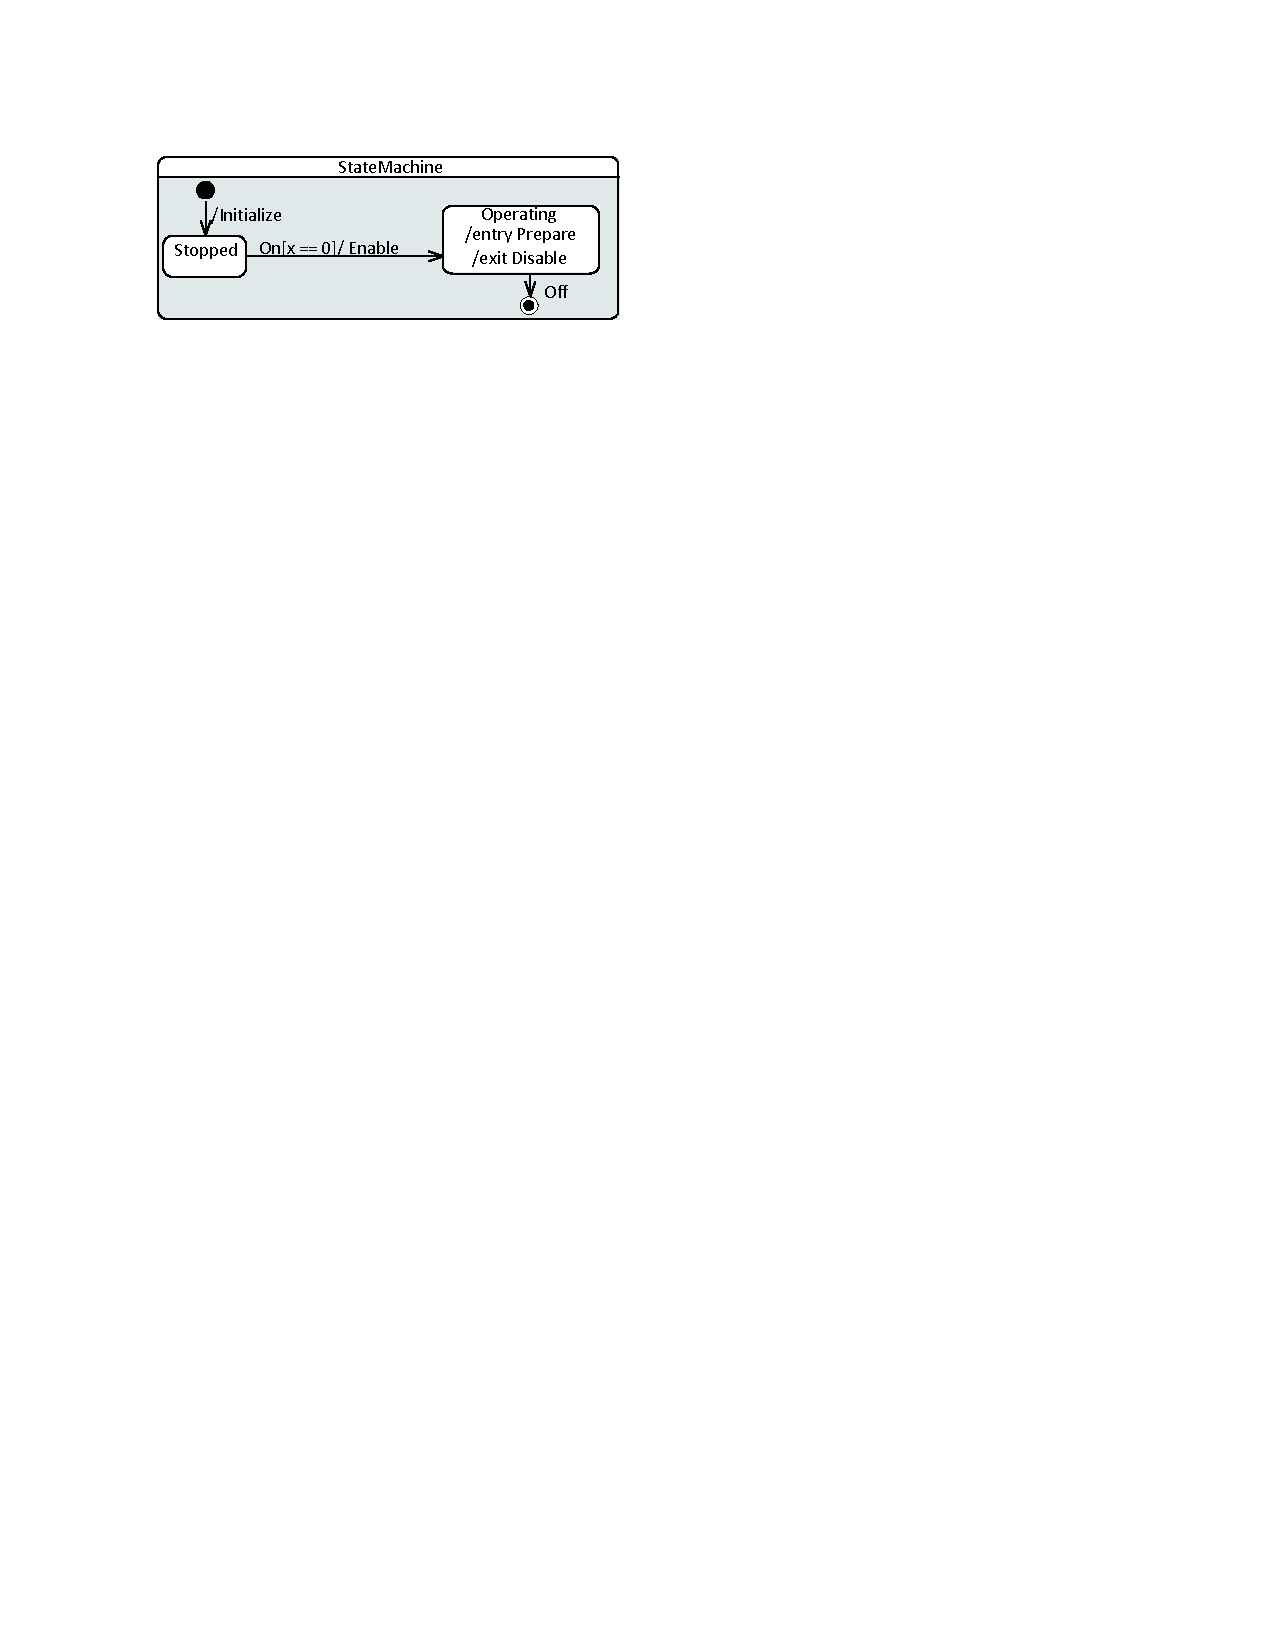
\includegraphics[clip, trim=2.5cm 22.5cm 10.5cm 2.5cm, width=0.4\textwidth]{figures/statemachine}
\caption{An example of SM for tracing table} 
\label{fig:statemachuine}
\end{figure}

\begin{table*}[]
\centering
\caption{Tracing table of state machine and class intermediate model}
\label{table:trace}
\begin{tabular}{|l|l|}
\hline
UML state machine concepts                                                 & UML class concepts                                     \\ \hline
Root::Client::StateMachine::TopRegion::Stopped (State)                     & Root::Client (Class)                                   \\ \hline
Root::Client::StateMachine (StateMachine)                                  & Root::Client::PerClass\_Client::StateMachine (Class)   \\ \hline
Root::Client::StateMachine::TopRegion::Stopped (State)                     & Root::Client::PerClass\_Client::Stopped (Class)        \\ \hline
Root::Client::StateMachine::TopRegion::Operating (State)                   & Root::Client::PerClass\_Client::Operating (Class)      \\ \hline
Root::Client::StateMachine::TopRegion::On (CallEvent)                      & Root::Client::PerClass\_Client::On (Class)             \\ \hline
Root::Client::StateMachine::TopRegion::Initialize(OpaqueBehavior)          & Root::Client::PerClass\_Client::Initialize (Operation) \\ \hline
Root::Client::StateMachine::TopRegion::Enable (OpaqueBehavior)             & Root::Client::PerClass\_Client::Enable (Operation)     \\ \hline
\end{tabular}
\end{table*}


The intermediate model is then used as input of a template-based object-oriented code generator. The use of an intermediate model facilitates the transformation from the SM to code and vice versa. Furthermore, the code generation process can use existing generators. Mappings from UML classes to object-oriented are trivial one-1-one. Listing \ref{lst:code-segment} shows a code segment generated from the SM in Figure \ref{fig:statemachuine}. The \ti{dispatchEvent} method implemented in the base composite state delegates an incoming event processing to its active sub-state. If the event is not accepted by the active sub-state, the composite state processes it. \ti{OnEntryAction} and \ti{OnExitAction} overwrite abstract methods which are defined in the base state class and called by the entry and exit methods, respectively. \ti{Stopped} accepts an \ti{On} event by implementing a corresponding \ti{processEvent} method. The transition method from the \ti{Stopped} to the \ti{Operating} state checks the guard condition by calling an associated method in the context class, then executes the transition action, changes the active state and finally enters the target state by calling entry. The machine enters the final state by setting the active state to null meaning that the behavior of the region containing the final state has completed. The generated code statements are intuitively similar to the UML SM semantics and it is easy to modify the behavior of the SM by code. For example, if we would like to change the default state, we only need to modify the \ti{setInitDefaultState} method by assigning the attribute \ti{activeSubState} to the attribute \ti{operating} that represent an instance of the state \ti{Operating}.

\subsubsection{Code generation}
\label{subsec:codegen}
\begin{minipage}{\linewidth}
\begin{lstlisting}[caption=A segment of C++ generated code, label=lst:code-segment]
class CompositeState: public State {
protected:
  State* activeSubState;
public:
bool dispatchEvent(Event* event) {
 if (activeSubState==NULL) {
  setIniDefaultState();
 }
 return activeSubState->
 dispatchEvent(event)||
this->processEvent(event);            
}}
StateMachine::StateMachine(Client* ctx){
  this->context = ctx;
  stopped = new Stopped(this, ctx);
  operating = new Operating(this, ctx);}
void StateMachine::setIniDefaultState(){
  this->context->Initialize();
  this->activeSubState = stopped;
  this->activeSubState->entry();}
bool StateMachine::transition(
        Stopped* state, On* event) {
 if(this->context->guard(event)){
  this->activeSubState->exit();
  this->context->Enable(event);
  this->activeSubState = this->operating;
  this->activeSubState->entry();
  return true;}
return false;}
bool StateMachine::transition(
    Operating* state, Off* event) {
  this->activeSubState->exit();
  //no action defined
  this->activeSubState = NULL;
return true;}
class Stopped: public State {
private:
  StateMachine* ancestor;
public: 
virtual bool processEvent(On* event) {
  return this->ancestor->transition(this,event);}
}
\end{lstlisting}
\end{minipage}

\subsection{Merging from modified code to UML SM}
This section describes the backward process. 

\subsubsection{Method Overall}
The generated code can be modified by adding/removing/changing states, transitions, actions. The modified generated code then needs to be reversed back to the SM to make the artifacts consistent. The overall method for backward transformation is shown in Figure \ref{fig:details}. The modified code is first verified by partly inspecting the code syntax and semantics to guarantee that the semantics of SM in the code is correct. This step is needed since not all of code modifications can be reversed back to the SM. The verification also produces an output (\ti{output2}) whose format is described later. If the intermediate model or the original SM is absent, a new intermediate model and a new SM are created. In the contrary, the intermediate model is used for generating the previous version of code or the previous code can be taken from control versioning systems. The previous code is also verified to have its output (\ti{output1}). \ti{Output1} and \ti{Output2} are then compared with each other to detect actual semantic changes which are about to be propagated to the original model. 

\begin{figure}
\centering
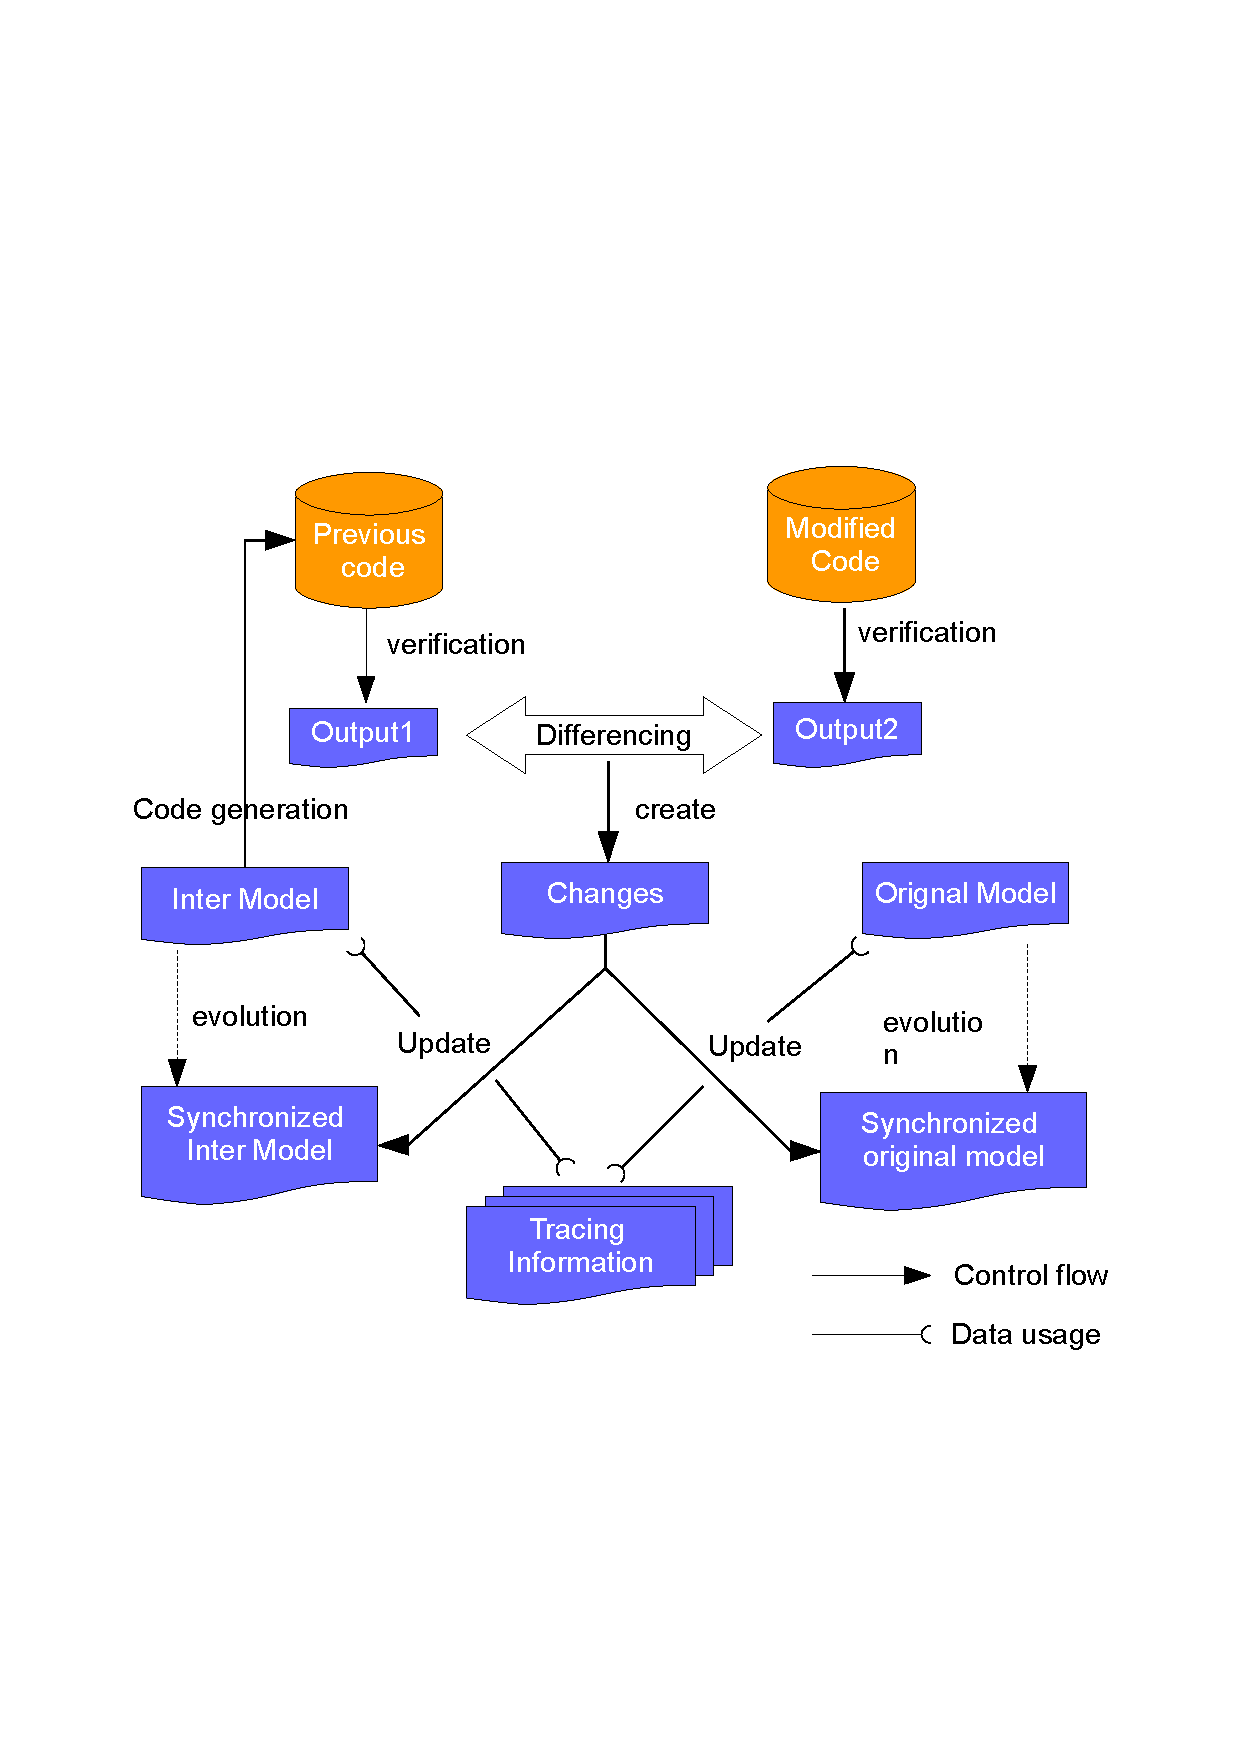
\includegraphics[clip, trim=1cm 7cm 0.1cm 7.8cm, width=0.47\textwidth]{figures/details.pdf}
\caption{Overall method for reversing code to state machine} 
\label{fig:details}
\end{figure}

\subsubsection{Semantic Verification}
The information contained by the output of the semantic verification is a list of event names, a list of state names, a list of transitions in which each has a source state, a target state, a guard function, an action function and an event represented in so called abstract syntax tree (AST) transition [15]. For example, Figure \ref{fig:transitions} presents the EMF \cite{gronback_eclipse_} representation of transitions in \tb{C++} AST in which \ti{IStructure} and \ti{IFunctionDeclaration} represent a structure and a function in \tb{C++}, respectively. Each state name is also associated with an ancestor state, an entry action, an exit action, a default sub-state and a final state. The output is taken by analyzing the AST. The verification process consists of recognizing different patterns. The pattern list is as followings:

\tb{State}: A state class inherits from the base state class or the composite base state class. For each state class, there must exist exactly one attribute typed by the state class inside another state class. The latter is the ancestor of the state class.

\tb{Composite state}: A composite state class (CSC) inherits from the base composite state. For each sub-state the CSC has an attribute typed by the associated sub-state class. The CSC also implements a method named \ti{setInitDefaultState} to set its default state. The CSC has a constructor is used for initializing all of its sub-state attributes at initializing time.

\ti{Entry action}: If a state has an entry action, its associated state class implements \ti{onEntryAction} that calls the corresponding action method implemented in the context class. If the state has outgoing \ti{triggerless} transitions, \ti{onEntryAction} appeals the \ti{triggerless} transition method of the ancestor state class following the entry action call.

\tb{Exit action}: Similar to the entry action pattern but implements \ti{onExitAction}.

\tb{Event processing}: If a state has an outgoing transition triggered by an event, the state class associated with the state implements the \ti{processEvent} method having only one parameter typed by the event class transformed from the event. The body calls the corresponding transition method of the ancestor class.
\ti{CallEvent} class: A call event class inherits from the base event class. The call event class contains attributes typed by the parameter types of the operation associated with the call event. This pattern is detected if the types of attributes of the event class match with the types of parameters of one of the methods in the context class. There is therefore an ambiguity for an event class to choose an associated operation if more than one operation detected matches the event class. Hence, this pattern poses a restriction that operations associated with events must either have different parameter types or different number of parameters. To overcome this issues, a naming convention used for \ti{CallEvent} classes is used. The event class name is prefixed with the associated operation name. If the event class name does not follow the naming convention, the reverse is refused. Another possible solution targeting this ambiguity is to have a user interaction in case of having more than one operation matching with the event. Having an interaction allows the pattern detection get rid of ambiguity and therefore provides appropriate SM models. A signal event is treated as a \ti{CallEvent} as previously described.

\tb{Time event}: A transition is triggered by a \ti{TimeEvent} if the state class associated with its source state implements the timed interface. The duration of the time event is detected in the transition method whose name is formulated as \ti{"transition" + duration}. 

\tb{Transition}: Transition methods are implemented in the ancestor class of the source state class. Two types of transition methods correspond to trigger and \ti{triggerless} transitions. Both \ti{parameterize} its source state class. The trigger transition method has an additional parameter typed by the event class associated with the event triggering the transition. The body of transition methods contains ordered statements including exiting the active state, executing transition action (effect), changing the active state to the target or null if the target is the final state, and entering the changed active state by calling entry. The body can have an if statement to check the guard of the transition. The transition action and the guard are optional. Several if/else statements can appear in a \ti{triggerless} transition method body.

\tb{Transition action/guard}: Transition actions and guards are implemented in the context class.

\begin{algorithm}[H]
  \caption{Semantic verification
    \label{alg:semantic-vefrification}}
  \begin{algorithmic}[1]
    \Require{AST of code and a list of state classes stateList}
	\Ensure{Output of semantic verification}
    %\Statex
    	\For {$s$ in $stateList$}
        	\For {$a$ in attribute list of $s$}
        		\If {$a$ and $s$ match child parent pattern}
        			put a and s into a state-to-ancestor map;
        		\EndIf
        	\EndFor
        	\For {$o$ in method list of $s$}
        		\If {$o$ is $onEntryAction$ || $o$ is $onExitAction$}		\State $verifyEntryExit(o)$; 	
        		\ElsIf {$o$ is $processEvent$} 
        			\State $verifyProcessEvent(o)$;
        		\ElsIf {$o$ is $setInitDefaultState$ \& $s$ is composite}
        			\State $verifyInitDefaultState(s)$;
        		\ElsIf {$o$ is timeout \& $s$ is a timedstate}
        			\State $verifyTimeoutMethod(o)$;
        			\State $verifyProcessEvent(s,o)$;
        		\EndIf	
        	\EndFor
    	\EndFor
  \end{algorithmic}
\end{algorithm}

Listing \ref{alg:semantic-vefrification} shows the algorithm used for verifying code semantics. Because of limited space, \ti{verifyEntryExit}, \ti{verifyProcessEvent}, \ti{verifyInitDefaultState}, \ti{verifyTimeoutMethod} and \ti{verifyProcessEvent} are not presented but they basically follow the pattern description as above. In the first step of the verification process, for each state class, it looks for an attribute typed by the state class, the class containing the attribute then becomes the ancestor class of the state class. The third steps checks whether the state class has an entry or exit action by looking for the implementation of the \ti{onEntryAction} or \ti{onExitAction}, respectively, in the state class to recognize the \ti{Entry/Exit} action pattern. Consequently, event processing, initial default state of composite state and time event patterns are detected following the description as above.  Figure \ref{fig:partition} shows the partitioning used for matching code segments to SM elements. Each partition consists of a code segment and the corresponding model element which are mapped in the backward direction. For instance, the \ti{Stopped} class in code is detected as a representation since it inherits from the base class \ti{State}.  
 
\begin{comment}
\begin{figure}
\centering
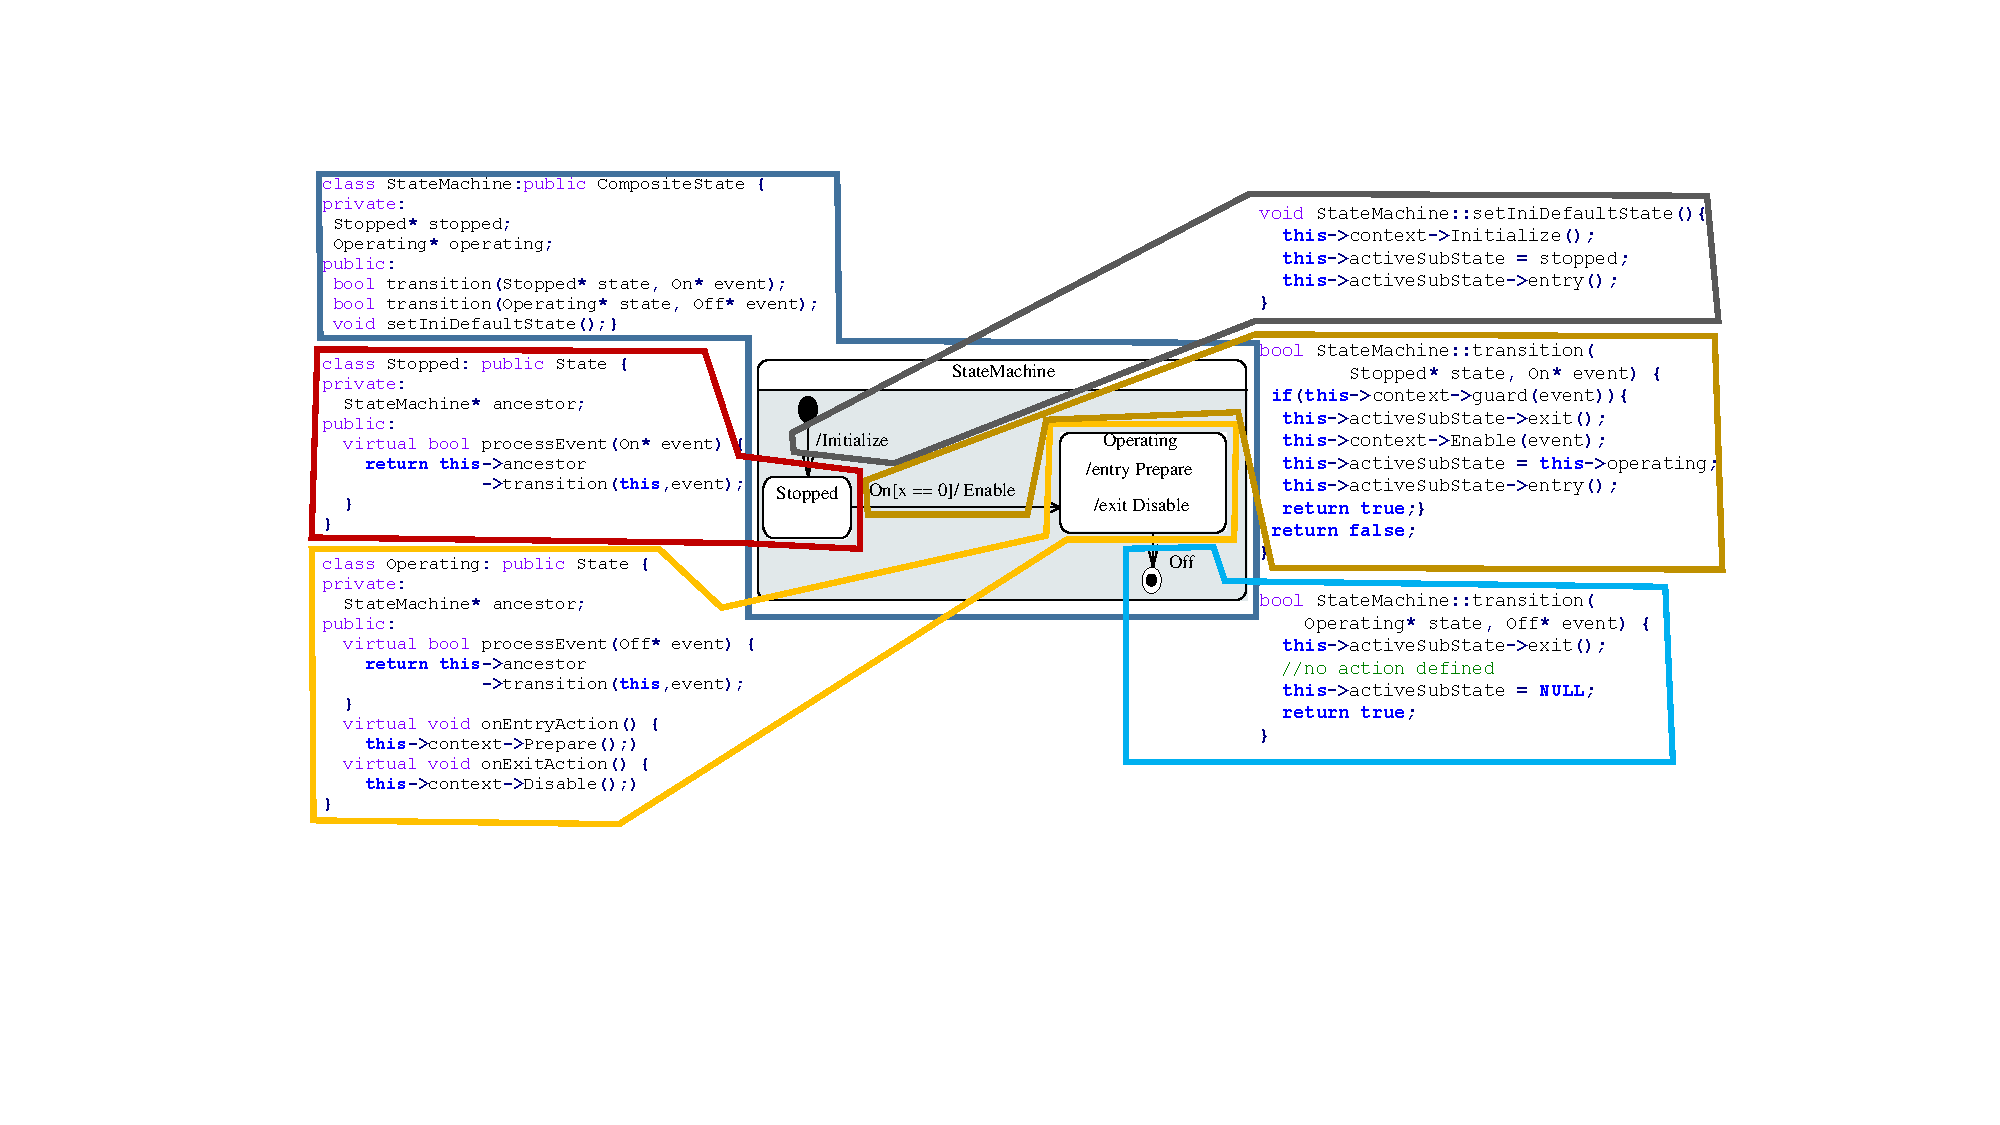
\includegraphics[clip, trim=1cm 4.8cm 0.1cm 0.8cm, width=0.75\textwidth]{figures/backwardmapping.pdf}
\caption{SM element-code segment mapping partition} 
\label{fig:partition}
\end{figure}
\end{comment}

\begin{figure}
\centering
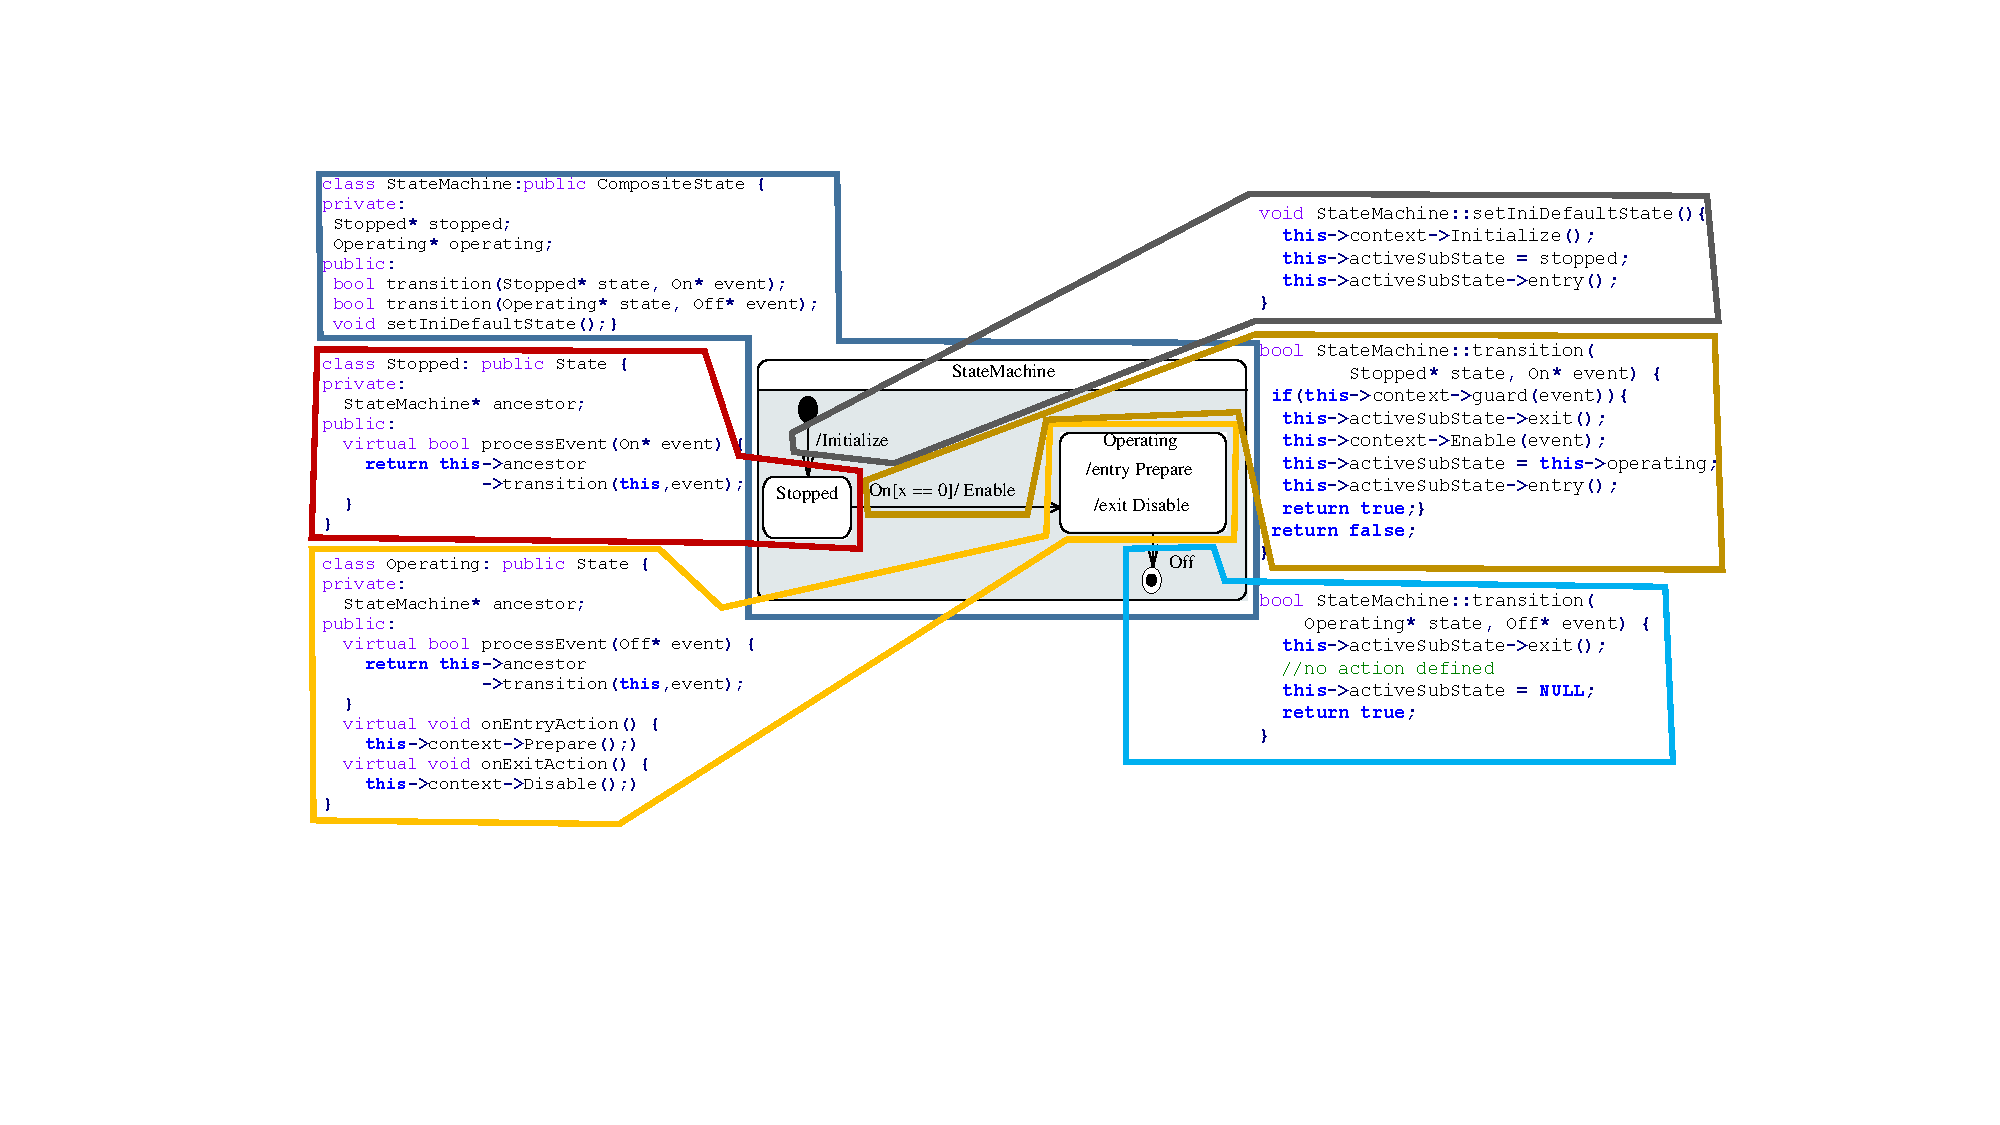
\includegraphics[clip, trim=5.2cm 5.1cm 0.1cm 2.8cm, width=0.52\textwidth]{figures/backwardmapping.pdf}
\caption{SM element-code segment mapping partition} 
\label{fig:partition}
\end{figure}

\begin{figure}
\centering
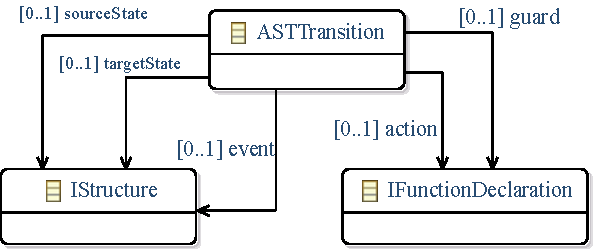
\includegraphics[clip, trim=0cm 0.06cm 0.0cm 0.08cm, width=0.3\textwidth]{figures/asttransition}
\caption{Transitions output from the verification of code} 
\label{fig:transitions}
\end{figure}

\subsubsection{Construction of SM from verification output}
If an intermediate model is not present, a new intermediate model and a new SM are created by a reverse engineering and transforming from the output of the verification process. The construction is straightforward. At first, states are created. Secondly, UML transitions are built from the AST transition list. Action/guard/triggering event of a UML transition is created if the associated AST transition has these.

\subsubsection{Updating the original SM from modified code}
In contrast to the previous sub-section, if an intermediate model is existing, it is also transformed into lists of states and transitions. The output of verification process and that of intermediate model transformation are compared to each other to detect the semantics changes of the modified code. The algorithm for detecting state and transition changes is shown in Listing \ref{alg:semantic-vefrification}.

The algorithm takes as input lists of state names, transitions, ancestor maps extracted from the intermediate model and the modified code, respectively. The algorithm results in lists of state names, transitions to be added/deleted/updated/moved. It first examines the list of state names extracted from the modified code $Lc$ for states that are not existing in the list of state names of the intermediate model $Li$ to be added to the added state list. If a state $c$ in $Lc$ is present in $Li$, $c$ is either added to the updated list if the ancestor states associated with $c$ in the intermediate model and the modified code are the same, or $c$ is considered as being moved to another ancestor state. Other states in $Li$ are added to the deleted state list. The transition change detection is similar to that of states but instead of checking by name, the source and target state names of transitions and the associated event name in $Tc$ and $Ti$ are used. Together with states and transitions but not presented in Listing \ref{alg:change-detect}, event changes are also detected similarly.

The changes detected by the algorithm are then used in a change propagation step which updates the original SM. Events, states and transitions are sequentially processed in order. The processing of deleted elements results in deleting corresponding elements in the SM. A deleted element in code is associated with an element in the intermediate model. As previously described, the mapping information for elements in code and the intermediate model is also stored in a table. Therefore, it is trivial to retrieve the model element in the intermediate model associated with the deleted element.

The found model element in turn helps identify the associated element in the SM by using the mapping table between the SM and the class model. For each deleted event in code, the associated event class in the class model and the event in the SM are deleted. Deleted states and transitions are similarly propagated. A deletion of a transition includes deleting its guard, triggers and transaction action. 
\begin{algorithm}[H]
  \caption{Change detection
    \label{alg:change-detect}}
  \begin{algorithmic}[1]
    \Require{$Li$, $Lc$, $Ti$, $Tc$, $mapI$, $mapC$ are lists of state names, transitions, ancestor map extracted from intermediate model and modified code, respectively}
	\Ensure{$adS$, $delS$, $uptS$, $movS$ are lists of added, deleted, updated and moved states respectively. $adT$, $delT$, $uptT$ are lists of added, deleted and updated transitions}
    %\Statex
    	\For {$c$ in $Lc$}
        	\If {!$Li$.contains($c$)} 
				\State adS.put(c);
        	\Else
				\If {$mapC$.get($c$) = $mapI$.get($c$)}
	    			\State uptS.put(c);
				\Else 
	    			\State $movS$.put($c$, $mapI$.get($c$), $mapC$.get($c$))	
                \EndIf
                	\State $Li$.remove($c$);
        	\EndIf
    	\EndFor
    	\For {$i$ in $Li$} 
        	\State $delS$.put($i$)
    	\EndFor
    	\For {$c$ in $Tc$}
        	\State $found$ = NULL
        	\For {$i$ in $Ti$}
				\If {$c$.source=$i$.source \& $c$.target=$i$.target \& $c$.event = $i$.event}
	    			\State $found$ = $i$;
              	\EndIf
             \EndFor 	
        	\If {$found$ != NULL} 
				\State $uptT$.put($c$);
				\State $Ti$.remove($found$);
        	\Else
				\State $adT$.put($c$);
        	\EndIf
    	\EndFor
    	\For {$t$ in $Ti$}
        	\State $delT$.put($t$);
    	\EndFor
  \end{algorithmic}
\end{algorithm} 
For each added event in code, an event is added to the class model and in turn to the SM. For each added state, its ancestor state is retrieved through the mapping tables, a new state is then created and attached to the ancestor. Entry and exit actions are also added to the new state afterward. A moved state is handled by looking for the associated state, the old and new ancestor state in the SM, and moving the associated state to the new ancestor. Each added transition is propagated by creating a new transition in the SM and retrieving source and target states from the mapping tables. An update is executed by looking in the mapping tables for elements in the SM associated with elements updated in code. It is worth noting that this algorithm detects a renaming of an event or state as a deletion followed by an addition. 


  
For example, assuming that we need to adjust the SM example shown in Figure \ref{fig:statemachuine}  by adding a guard to the transition from \ti{Operating} to the final state. The adjustment can be ordered by either modifying the SM model or the generated code. In case of code, the associated transition function in Listing \ref{lst:code-segment} is edited by inserting an if statement which calls the guard method implemented in the context class. The transition function becomes as in Li. The algorithm in Listing \ref{alg:change-detect} adds the transition function into the updated list since it finds that the source state, the target state and the event name of the transition is not changed. By using mapping information in the mapping table, the original transition in the SM is retrieved. The guard of the original transition is eventually created. 	






\section{implementation}
\label{sec:implementation}
The proposed approach is implemented in a prototype existing as an extension of the Papyrus modeler [4]. Each state machine is created by using a state machine diagram and contained in a component. Low-level processing of state machine actions is directly embedded by a block of code written specific programming languages such as C++/JAVA in the state machine. C++ code is generated by the prototype but other object-oriented languages are easily generated. The code generation consists of transforming the state machine to UML classes and eventually to code by a code generator following the proposed approach. In the reverse direction, code pattern detection is implemented as described in the previous section to verify state machine semantics in code. If the generated code is modified, two options are supported by the prototype interface to make the state machine and code consistent again. One is to create a new state machine from the modified code in the same Eclipse project and the other one is to update the original state machine by providing as input the intermediate model and the state machine in a dialog.
\section{Experiments}
\label{sec:experiments}
In order to evaluate the proposed approach and the prototype, we answer two questions related to two laws of RTE \cite{foster_combinators_2007}. 

\tb{RQ1}: A state machine \ti{sm} is used for generating code. The generated code is reversed by the backward transformation to produce another state machine \ti{sm'}. Are \ti{sm} and \ti{sm'} the same? In other words: whether the code generated from UML state machines model can be used for reconstructing the original model.

\tb{RQ2}: A state machine sm is used for generating code. The generated code is modified by adding/deleting/modifying elements such as states, transitions, or events. The modified code is then reversed by merging changes to sm. Are modifications in the modified code propagated to sm?

This section reports our experiments targeting to the two questions. Two types of experiments are conducted. For each type, the number of elements in models are taken into account by a JAVA program. Figure \ref{fig:strategy1} and Figure \ref{fig:strategy2} show the evaluation methodologies to answer \tb{RQ1} and \tb{RQ1}, respectively. Additionally, the time complexity and performance analysis of our approach is also presented. Results of a lightweight experiment on the semantic conformance of runtime execution of the generated code are also shown afterward.

\begin{figure}
\centering
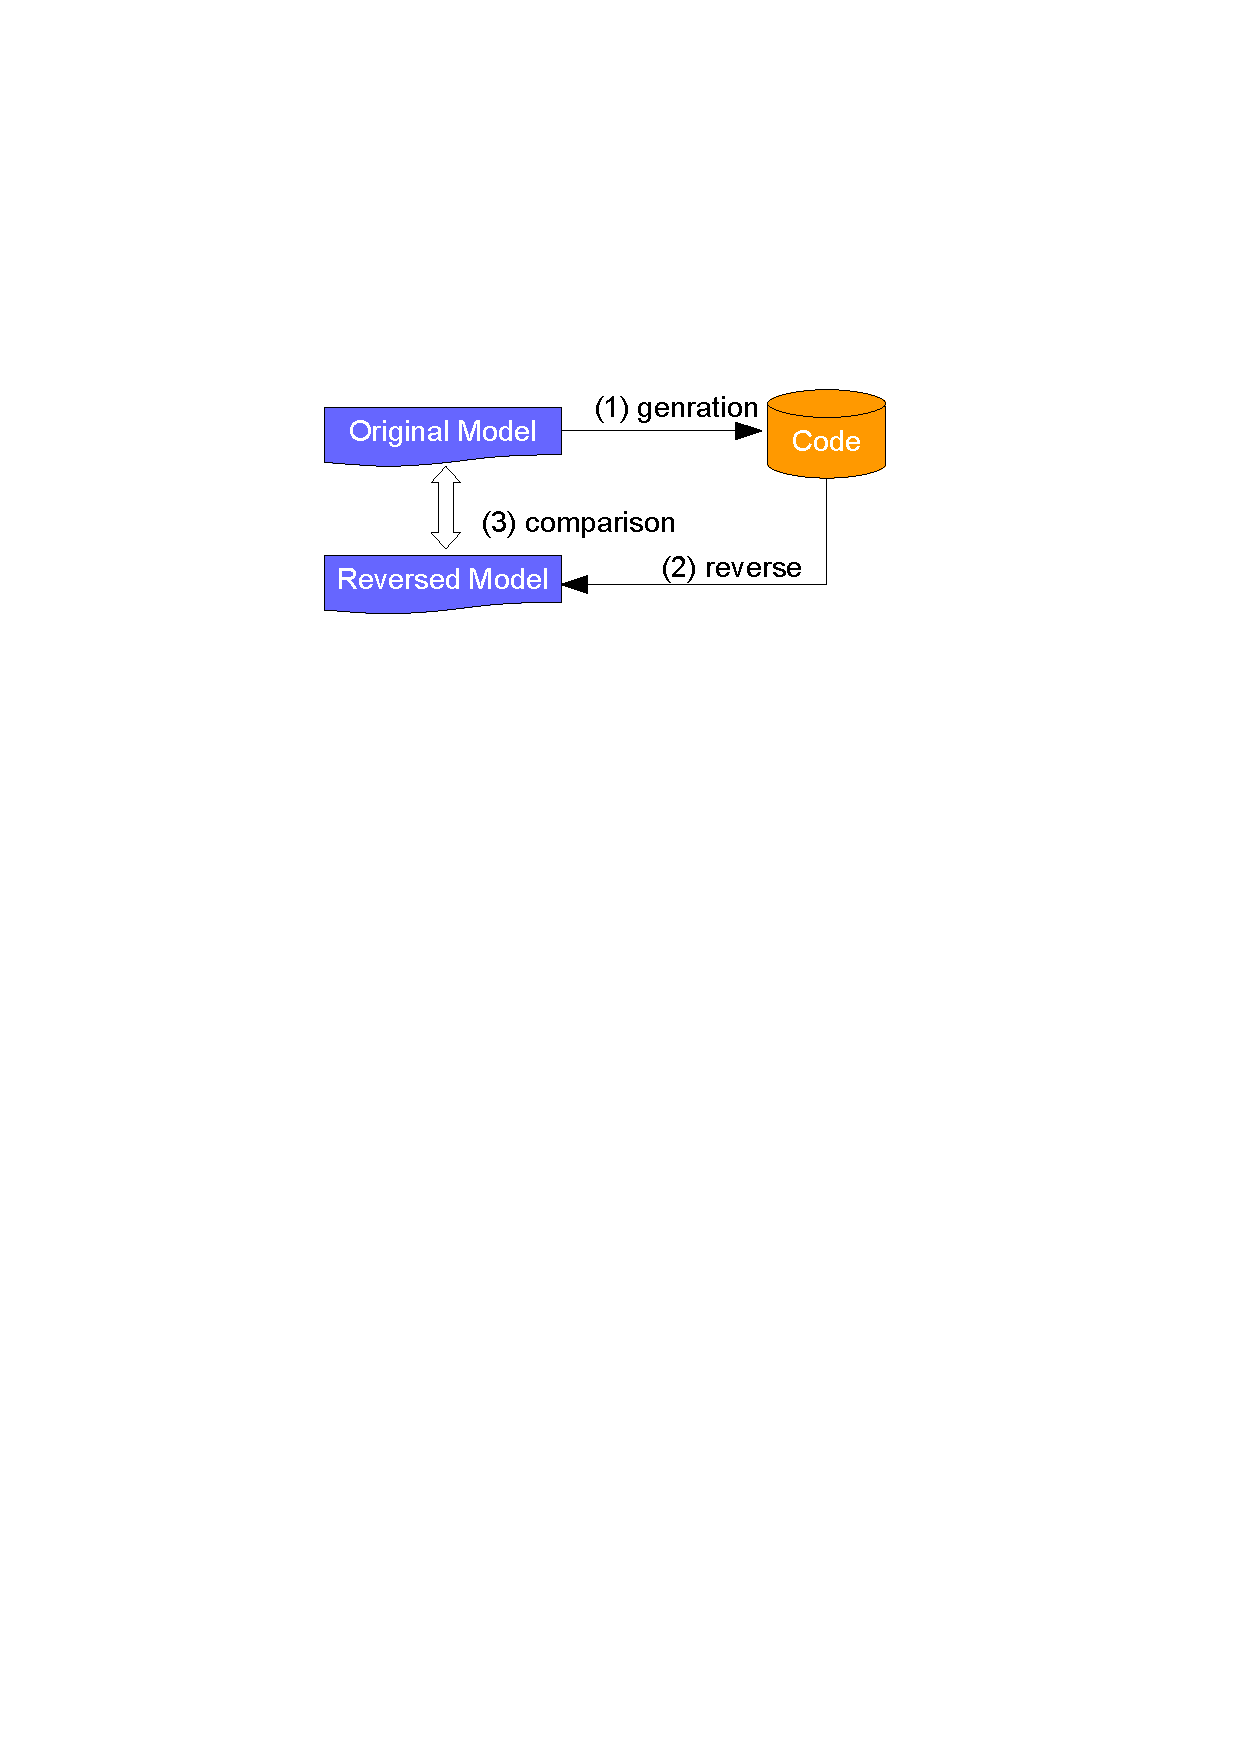
\includegraphics[clip, trim=5.5cm 19cm 5.5cm 6cm, width=0.3\textwidth]{figures/strategy1}
\caption{Evaluation methodology to answer RQ1} 
\label{fig:strategy1}
\end{figure}

\begin{figure}
\centering
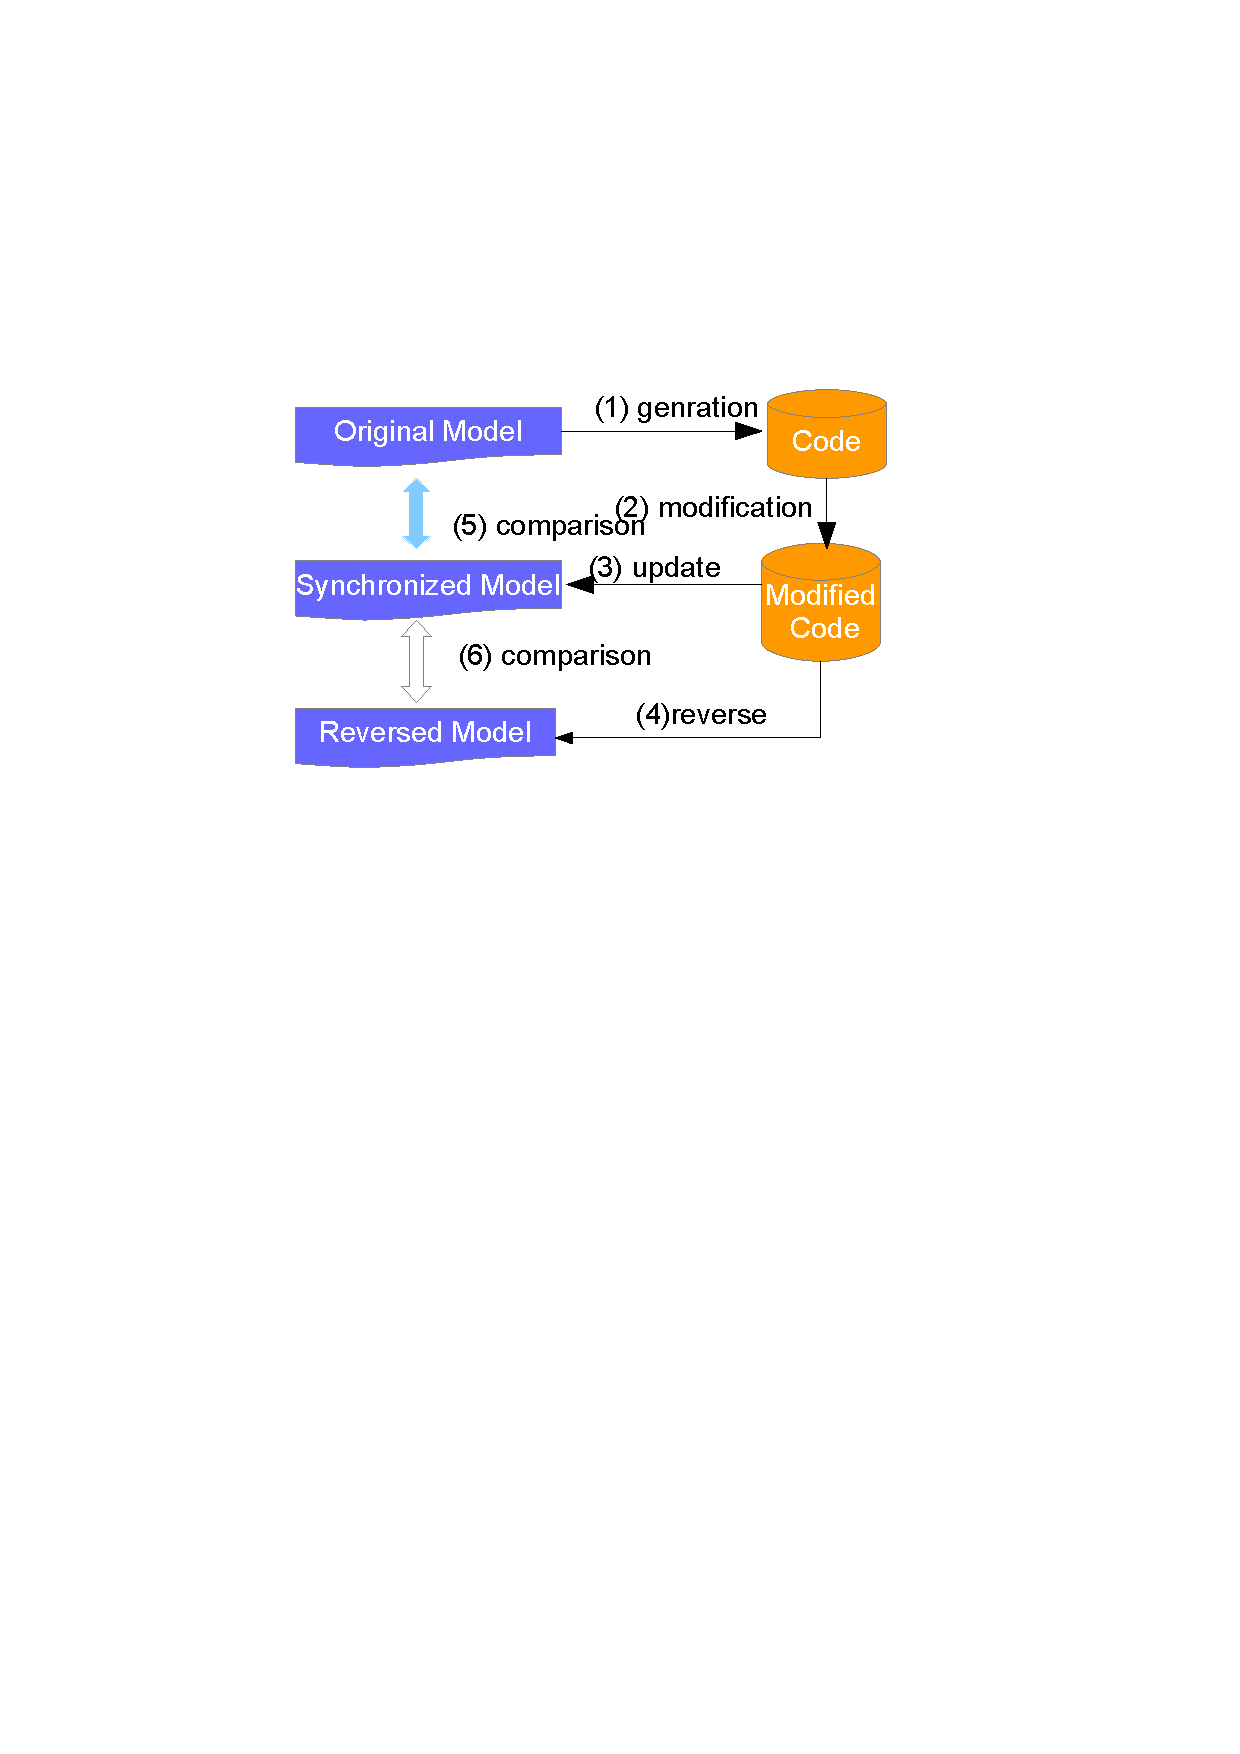
\includegraphics[clip, trim=4.5cm 16.5cm 5.5cm 6.5cm, width=0.3\textwidth]{figures/strategy2}
\caption{Evaluation methodology to answer RQ2} 
\label{fig:strategy2}
\end{figure}

Furthermore, in software development projects, some traditional programmers might want to practice with code in a traditional way and some MDE developers may prefer working with models. Therefore, it is necessary to compare the development/maintenance cost between the two practices by comparing the number of steps needed to do the same action. 


\subsection{Reversing generated code}
This experiment is targeting \tb{RQ1}. 300 hierarchical state machines are randomly automatically generated. Each of these has 80 states including atomic and composite states, and more than 234 transitions. The number of elements is unrealistically big but it is artificially used to show the scalability of the approach. The number of lines of generated code for each machine is around 13500. Names of the generated states are different. An initial pseudo state and a final state are generated for each composite state and containing state machine. Other elements such as call events, time events, transition/entry/exit actions and guards are associated with an appearance probability sensing that if a random number is less than the probability, the element associated with the probability is generated. For each generated call event, an operation is generated in the context class which is also generated. The duration is also generated for each time event. 


\begin{table}
\centering
\caption{Set-up information for model generation}
\label{table:setup}
\begin{tabular}{|l|l|}
\hline
Description                                     & Value            \\ \hline
Number of generated states                      & 80               \\ \hline
Number of generated transitions                 & \textgreater 234 \\ \hline
Probability of having an event for transition   & 0.8              \\ \hline
Probability of having CallEvent for transition  & 0.7              \\ \hline
Probability of having an entry/exit action for state & 0.7              \\ \hline
Probability of having a transition action and guard       & 0.7              \\ \hline
\end{tabular}
\end{table}

The set up information for the SM generation is shown in Table \ref{table:setup}. Code is generated from each state machine. The generated code is reversed to a state machine. The latter is then compared to the original one by using information of SM such as the number of states, transitions. 

\begin{table}
\centering
\caption{Model results of generation and reverse}
\label{table:law1-resultat}
\begin{tabular}{|l|l|l|l|l|}
\hline
Test ID & AS & CS & T & Is reverse correct? \\ \hline
1       & 47 & 33 & 234 & Yes                 \\ \hline
2       & 42 & 38 & 239 & Yes                 \\ \hline
3       & 43 & 37 & 238 & Yes                 \\ \hline
..      & .. & .. & .. & Yes                 \\ \hline
300       & 41 & 39 &240 & Yes                 \\ \hline
\end{tabular}
\end{table}
 
 
\begin{comment}
\begin{table*}[]
\centering
\caption{MODEL RESULTS OF GENERATION AND REVERSE}
\label{table:law1-resultat}
\begin{tabular}{|l|l|l|l|l|l|l|l|l|l|l|l|l|l|}
\hline
Test ID & AS & CS & D  & T   & EA & ExA & TA  & CE  & TE & G   & I  &    & Is reverse correct? \\ \hline
1       & 47 & 33 & 8  & 234 & 53 & 50  & 149 & 145 & 40 & 147 & 34 & 25 & Yes                 \\ \hline
2       & 42 & 38 & 8  & 239 & 52 & 59  & 165 & 145 & 36 & 133 & 39 & 31 & Yes                 \\ \hline
3       & 43 & 37 & 7  & 238 & 54 & 59  & 159 & 141 & 34 & 145 & 38 & 28 & Yes                 \\ \hline
..      & .. & .. & .. & ..  & .. & ..  & ..  & ..  & .. & ..  & .. & .. & Yes                 \\ \hline
300       & 41 & 39 & 10 & 240 & 56 & 55  & 165 & 142 & 37 & 151 & 40 & 33 & Yes                 \\ \hline
\end{tabular}
\end{table*}
\end{comment}

Table \ref{table:law1-resultat} shows some of the generated models which have the same information as the models created by doing the backward process of the generated codes. The number of atomic states (\tb{AS}), composite states (\tb{CS}), transitions (\tb{T}) are shown in Table \ref{table:law1-resultat}. The results of this experiment show that the proposed approach and the implementation can successfully do code generation from state machines and reverse. The answer to \tb{RQ1} is Yes. 

\subsection{Change propagation} 
A state machine (model level) describing Java Thread life-cycle \cite{_java_thread} and another one representing a telephone presented in \cite{Specification2007} are manually created. For each SM code is generated. Code is then manually modified by several actions described in Table \ref{table:cost}. The original SM is updated by doing a backward process from the modified generated code with the presence of the intermediate and original model. The updated SM is in turn compared with the SM created by the reverse engineering (see Fig. \ref{fig:strategy2}). 

\begin{table}
\centering
\caption{Change propagation experimental results}
\label{table:change-propa}
\begin{tabular}{|l|l|l|l|l|}
\hline
Test ID & Changes & Original & Updated & Reversed \\ \hline
1       &         &          &         &          \\ \hline
2       &         &          &         &          \\ \hline
3       &         &          &         &          \\ \hline
4       &         &          &         &          \\ \hline
\end{tabular}
\end{table}

\subsection{Time complexity and performance}
We are interested in knowing which element type among state, transition and event dominates the running time of the reverse engineering in case of creating new SM from code. To analyze the time complexity, we consider two tasks: semantic verification and SM construction from the verification output. Let us use the following parameters of the input SM used in code generation: $n_{s}$ = number of states, $n_{t}$ = number of transitions, $n_{ce}$ = number of call events, $n_{te}$ = number of time events, $n_{a}$ = number of actions and guards including entry/exit/transition actions and guards which are all implemented in the context class. 

For each state, the semantic verification consists of several phases as followings: (1) detecting composite/sub-state pattern, (2) loop over all methods of a state class, (3) detecting entry action pattern, (4) detecting exit action pattern, (5) detecting processing \ti{CallEvent}, (6) detecting processing \ti{TimeEvent}, and (7) detecting default state pattern. 
\begin{comment}
\begin{itemize}
  \item Detecting composite/sub-state pattern: $C_{childParentPattern} = ns^2 = O (ns^2)$.
  \item Loop over all methods of a state class: $CfindAllStateOperation = ns + nce + nt$. 
  \item Detecting entry action pattern: $Centry = na + CverifyTransition + CfindFunctionDefinition 
      = 6ns + 6nce + 5na + nt$
   \item Detecting exit action pattern: Cexit = 3nce + 3ns + 3na + nt
   \item Detecting processing CallEvent: CprocessEvent = 7nce + 6ns + 2nt + 2na 
   \item Detecting processing TimeEvent: CprocessTimeEvent = 6nce + 6ns + 2nt + 2na
   \item Detecting default state pattern: CsetInitDefaultState = 3nce + 3ns + nt + na
\end{itemize}

\begin{itemize}
  \item Detecting composite/sub-state pattern
  \item Loop over all methods of a state class
  \item Detecting entry action pattern
   \item Detecting exit action pattern
   \item Detecting processing \ti{CallEvent}
   \item Detecting processing \ti{TimeEvent}
   \item Detecting default state pattern
\end{itemize}
\end{comment}
Since the space is limited, we cannot present the detail of the complexity of each phase. To sum up, the semantic verification has a worst-case complexity $C_{1} = n_{s}(n_{s^2} + 9n_{t^2} + 6n_{t}n_{s} + 2n_{a}n_{ce}) = O (n_{s^3}) + O (n_{t}n_{s^2}) + O (n_{s}n_{t^2}) = O (n^3)$ with $n = max (n_{t}, n_{s})$. The worst-case occurs if a state can accept all incoming events and all transitions have the same source state. This is indeed unrealistic.

The SM construction from the verification output has a worst-case time complexity $C_{2} = O (n_{s^2}) + O (n_{s} n_{t}) = O (n_{^2})$. Therefore, the reverse engineering has a worst-case complexity of $O (n^3)$ with $n = max (n_{s}, n_{t})$.

To analyze the performance of reverse engineering, we randomly generate 5 models with base set up information in which the numbers of states and transitions are 20 and 50, respectively. We use a Dell Latitude E554 laptop with a 2.1GHz Intel Core i7 with 16 Gb of RAM. The running time of the reverse for the generated code associated with these models is measured. To analyze the impact of state and transition to the reverse performance, we change the set up information by increasing either the number of states or transitions, and keep intact the other. The increase is of 5, 10, 15, and so on. The models resulting from the modifications are used for generating code. The running time of reverse engineering the new generated code is measured. For each measurement, three times are computed, the median of these measured values are retained. 

\begin{table}
\centering
\caption{Time measurements}
\label{table:time-measurment}
\begin{tabular}{|l|l|l|l|}
\hline
Increase & Original & State  & Transition \\ \hline
5        & 64557    & 78021  & 62271      \\ \hline
10       & 64557    & 83025  & 68374      \\ \hline
15       & 64557    & 96761  & 64176      \\ \hline
20       & 64557    & 118879 & 71728      \\ \hline
25       & 64557    & 132763 & 73445      \\ \hline
30       & 64557    & 153120 & 75314      \\ \hline
35       & 64557    & 163538 & 78647      \\ \hline
40       & 64557    & 185361 & 81547      \\ \hline
\end{tabular}
\end{table}

Table \ref{table:time-measurment} shows the increase of the number of instances for states and transitions and the execution time of the original and modified models. The results show that when the number of states has more impact to the performance overall than the number of transitions. Figure \ref{fig:graph} also shows clearer the comparison of performance between the original model, the models modified by adding states and transitions. When the number of added states grows, the running time for reverse also grows quickly. Whereas, in case of transitions, the difference is small and not clear as we analyze that the worst-case complexity never occurs.

\begin{figure}
\centering
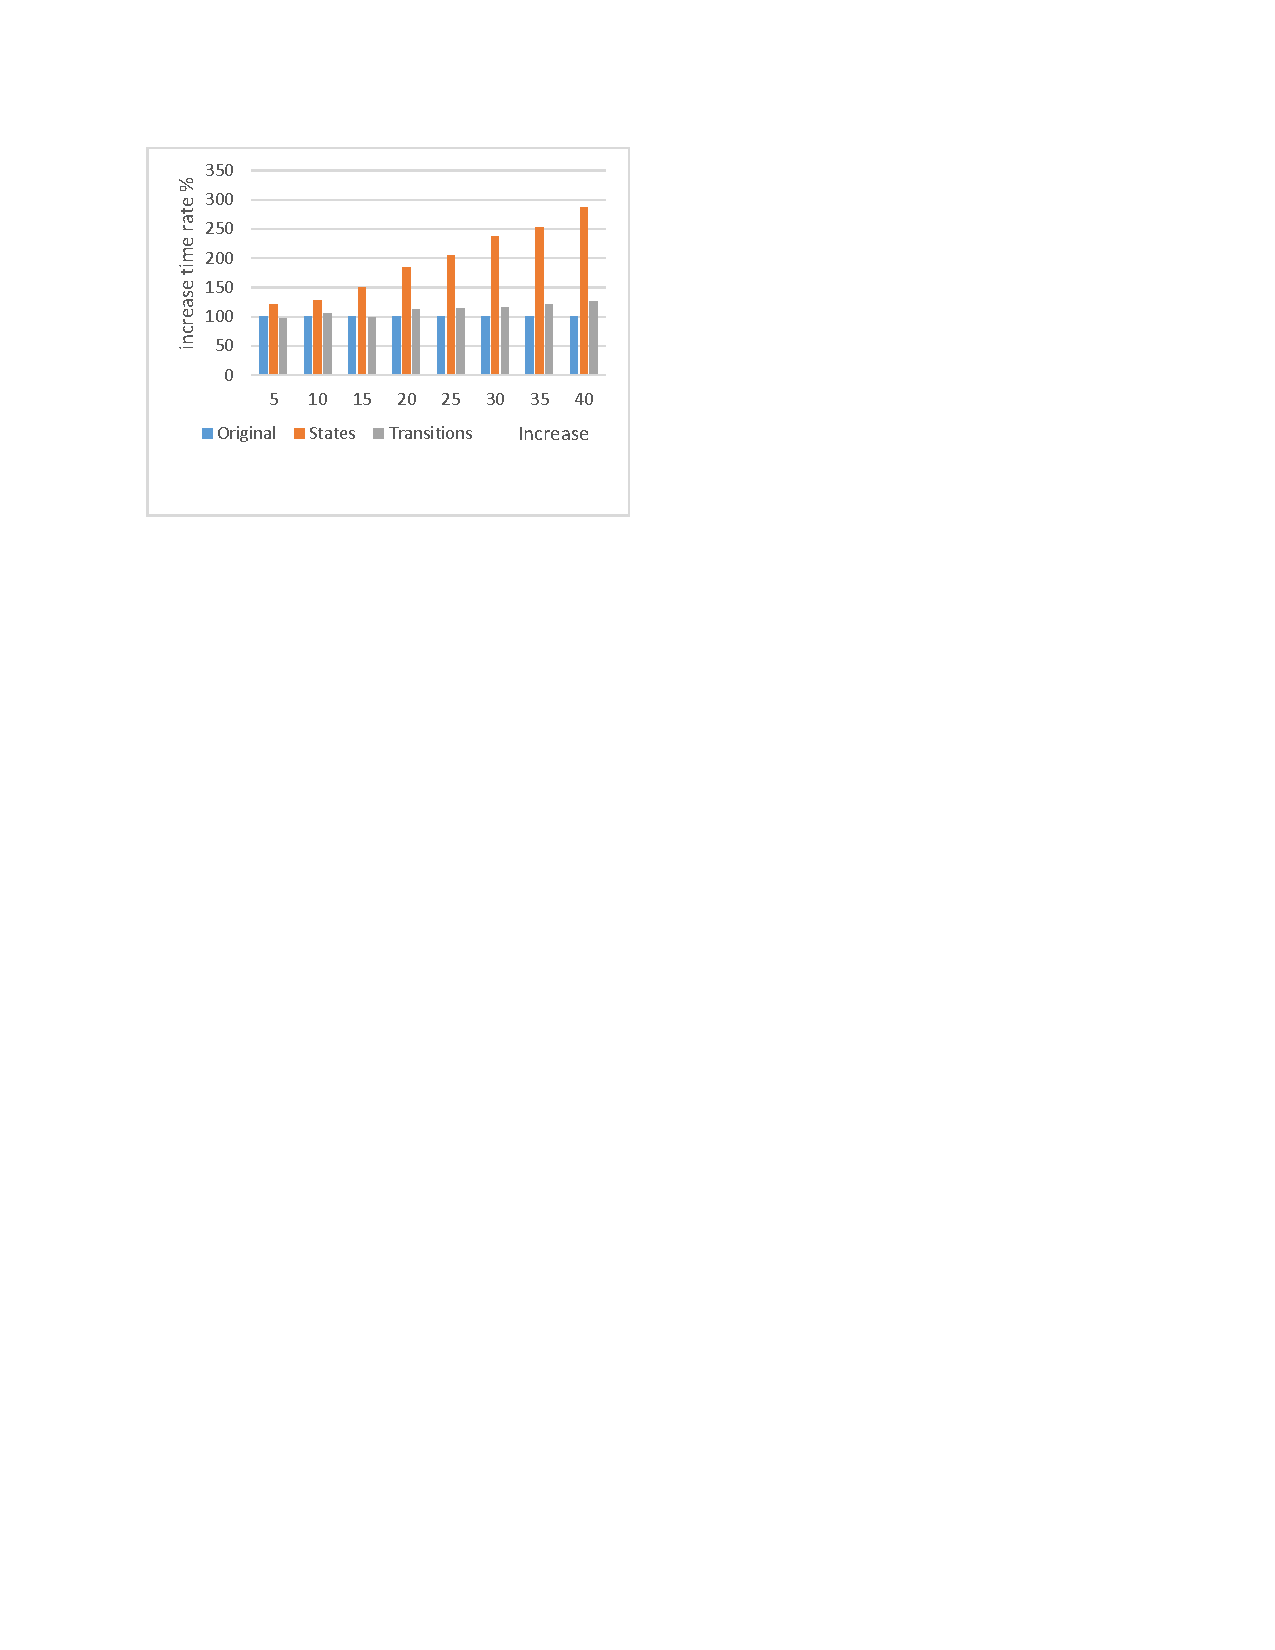
\includegraphics[clip, trim=3cm 20.5cm 11cm 2.6cm, width=0.5\textwidth]{figures/graph}
\caption{Impact comparison between states and transitions} 
\label{fig:graph}
\end{figure}

\subsection{Semantic conformance of runtime execution}
To evaluate the semantic conformance of runtime execution of generated code, we use a set of examples provided by Moka [XXX] which is a model execution engine offering Precise Semantics of UML Composite Structures \cite{OMG2015}. We compare the entered-ordered state list, which is obtained by simulating a state machine with the engine, with the state list obtained by the runtime execution of the generated code of the same state machine. The generated code is semantic-conformant if both of the lists are the same. [To be continued]

\subsection{Development/maintenance cost}
\label{subsec:cost}
To compare the development/maintenance cost, we investigate steps needed in generated code and models having the equivalent semantics. For example, to add a state, on one hand, two steps are needed in diagrams including (1) specifying the parent state and (2) dragging \& dropping the state notation to that parent. On the other hand, three code modifications are (1) create a state class inheriting from the base state and its constructors, (2) add to the parent state class an attribute, and (3) add a line of code to initialize the state attribute in the parent state constructor. Table \ref{table:cost} shows the number of steps needed for each operation. In this table, model manipulations are the winner in most of cases because of graphical representation advantages but code manipulations are still useful and comparable.

\begin{table}
\centering
\caption{Cost comparison}
\label{table:cost}
\begin{tabular}{|l|l|l|}
\hline
Description                                     & Model & Code \\ \hline
Add a state                                     & 2     & 3    \\ \hline
Add a transition                                & 3     & 3    \\ \hline
Add entry/exit action                           & 2     & 2    \\ \hline
Add transition action                           & 2     & 2    \\ \hline
Update action                                   & 1     & 1    \\ \hline
Redirect target state of a transition           & 1     & 1    \\ \hline
Create a call event to a transition & 3     & 6    \\ \hline
Create a time event to a transition & 3     & 5    \\ \hline
Delete a state                                  & 2     & 2    \\ \hline
Delete a transition                             & 1     & 3    \\ \hline
Delete entry/exit action                        & 1     & 2    \\ \hline
Delete transition action                        & 1     & 2    \\ \hline
Delete a call event                             & 2     & many \\ \hline
Delete a time event                             & 2     & many \\ \hline
\end{tabular}
\end{table}

In software development, programmers might modify the generated code, the modifications might violate structures of code or SM semantics. To resolve this issue, as previously described, we provide a semantic verification that partly and loosely inspects the AST of generated code. This inspection approach always reverses the code to the SM as well as the code is state machine-compliant even though the code is not compiled. This approach is very useful in practice in which programmers might partly modify code, automatically update the original SM by our RTRIP, and automatically re-generate state machine-compliant code into the remaining application code. This re-generation does no more than completing missing elements in code meaning that all previous changes are preserved. This practice is also limitedly supported by Fujaba \cite{KNNZ99_2_ag} in which activity and collaboration diagrams are partly synchronized with JAVA.




\section{Conclusion}
\label{sec:conclusion}
This paper presented a novel approach to round-trip engineering from UML state machines to code and back. The forward process of the approach is based on different patterns transforming UML state machine concepts such as states, transitions and events into an intermediate model containing UML classes. Object-oriented code is then generated from the intermediate model by existing code generators for programming languages such as C++ and JAVA. In the backward direction, code is analyzed and transformed into an intermediate whose format is close to the semantics of UML state machines. UML state machines are then straightforwardly constructed or updated from the intermediate format. 
 
The paper also showed the results of several experiments on different aspects of the proposed approach with the tooling prototype. Specifically, the experiments on the correctness of, the performance of, the semantic conformance of code generated by, and the cost of system development/maintenance using the proposed round-trip engineering are conducted. Although, the reverse direction only works if manual code is written following pre-defined patterns, the semantics of state machines is explicitly and intuitively present and easily to follow.

While the semantic conformance of code generated is critical, the paper only showed a lightweight experiment on this aspect. The reason is that the implementation of the prototype takes a lot of time. A systematic evaluation is therefore in future work. Furthermore, as evaluated in [7], the approach inheriting from the double-dispatch trades a reversible mapping for a slightly larger head. The reverse does not work concurrent state machine and several pseudo-states. Hence, future work should resolve these issues.

%\input{sections/ack}
\bibliographystyle{abbrv}
\bibliography{refs}

\end{document}